\documentclass[UTF8,fontset=fandol,a4paper,zihao=-4]{ctexart}
\usepackage[a4paper,margin=2.5cm]{geometry}
\usepackage{amsmath,amssymb,amsthm,bm,booktabs,array,longtable,graphicx,float}
\usepackage{enumitem,xcolor,listings,hyperref,fancyhdr}
\hypersetup{hidelinks,pdftitle={有界示向误差下无线电干扰源的覆盖认证搜索与快速清除},pdfauthor={}}
\setlength{\parindent}{2em}
\setlength{\parskip}{0.15em}
\linespread{1.15}
\setlist{itemsep=0.2em,topsep=0.3em,parsep=0pt}
\pagestyle{fancy}\fancyhf{}\fancyfoot[C]{\thepage}
\renewcommand{\headrulewidth}{0pt}
\newtheorem{theorem}{结论}
\newtheorem{proposition}{命题}
\DeclareMathOperator*{\argmin}{arg\,min}
\DeclareMathOperator{\conv}{conv}
\newcommand{\dd}{\mathrm{d}}
\newcommand{\norm}[1]{\left\lVert#1\right\rVert}
\newcommand{\cross}[2]{\operatorname{cross}(#1,#2)}
\newcommand{\disk}{\mathcal D}
\newcommand{\poly}{\mathcal P}
\lstset{basicstyle=\ttfamily\fontsize{7.5}{9}\selectfont,breaklines=true,breakatwhitespace=false,
  columns=fullflexible,keepspaces=true,showstringspaces=false,frame=single,
  numbers=left,numberstyle=\tiny,numbersep=5pt,tabsize=4,
  keywordstyle=\color{blue!55!black},commentstyle=\color{black!65},
  stringstyle=\color{green!35!black},captionpos=t,xleftmargin=1.5em}
\newcommand{\ExperimentRuns}{4430}
\newcommand{\QThreeTime}{310.67}
\newcommand{\QThreeBaseline}{515.57}
\newcommand{\QThreeGain}{39.74}
\newcommand{\QFourTime}{803.28}
\newcommand{\QFourBaseline}{1046.74}
\newcommand{\QFourGain}{23.26}

\setlength{\emergencystretch}{3em}
% Gains are percentage reductions of paired-group mean T/N.
\newcommand{\EnhancedQThreeTime}{275.68}
\newcommand{\EnhancedQThreeGain}{12.48}
\newcommand{\EnhancedQFourTime}{797.76}
\newcommand{\EnhancedQFourGain}{1.72}
\newcommand{\EnhancementRuns}{3080}
\newcommand{\ContractedRadius}{1200.00}

\newcommand{\RingSelectedTime}{272.71}
\newcommand{\RingControlTime}{275.09}
\newcommand{\RingSaving}{2.377}
\newcommand{\RingLowerCI}{1.608}
\newcommand{\RingUpperCI}{3.145}
\newcommand{\RingFaster}{353}

\begin{document}
\begin{center}
{\LARGE\bfseries 有界示向误差下无线电干扰源的\\覆盖认证搜索与快速清除\par}
\vspace{0.6em}
{\small 研究与复核稿：官方模拟器测试已按要求搁置，非可直接提交版本}
\end{center}
\begin{center}\bfseries 摘要\end{center}
无线电干扰源数量、接收半径以及定向源的发射方向均未知，因而快速定位不仅是多条示向线求交，还必须解决误差约束、全区域发现与正确停止三个问题。本文采用“确定性覆盖保证正确性、观测驱动调度降低耗时”的统一框架。

针对问题一，将每次示向度转为正向楔形半平面约束，给出空集、有界和无界情形的判别及顶点对直径算法。构造由合法测向观测实现的边长36米等边三角形反例，证明直径为区域直径的圆不一定覆盖区域；以最小包围圆半径代替区域直径作为一次清除判据。

针对问题二，利用首次接收到信号隐含的接收半径下界，推导无需已知目标距离的三圆交候选区域。以交会夹角与距离共同刻画测向条件，并以候选点的后验可行域包围圆半径进行采样极小极大评分，区分可证明的接收安全性与启发式的最优性。

针对问题三，先构造900米覆盖的七点骨架并证明该覆盖半径下七点达到点数下界，再将六点环半径收缩为1200米，利用精确覆盖公式保留31.10米接收余量；收缩环旨在减少行程，实际总耗时收益仍需由同口径合成实验检验。针对问题四，用含圆域外点的31点三角格及凸包半平面性质保证任意发射方向不漏检，构造逐点不可删反例，并从实际位置滚动优化剩余骨架顺序。两问均维护逐频道完成证书；局部定位保留有限测向和完整光学覆盖后备。

在明确声明分布与固定地点误差的本地环境中，基础对照执行\ExperimentRuns{}次运行；另用\EnhancementRuns{}次隔离种子的运行评估本轮增强。每问500个新随机世界上，Q3平均单源总耗时为\EnhancedQThreeTime{}秒，较同世界基础集成策略降低\EnhancedQThreeGain\%；Q4为\EnhancedQFourTime{}秒，降低\EnhancedQFourGain\%。所列运行均全清；静态2-opt和区间自适应测点因完整耗时未改善而未被默认采用。所有结果均非官方成绩；正式日志和参赛队人工核验仍缺失。

\noindent\textbf{关键词：}有界误差；交会定位；最小包围圆；覆盖证书；主动测向；定向源搜索
\newpage

\section{问题理解、目标与证据边界}
\subsection{四问之间的依赖关系}
题目给定半径1800米的目标圆域，最多20个频道、每频道至多一个静止干扰源；在问题三、四中目标总数为10至16但不向程序公开。每次检测只报告无信号、近源或带误差的示向度，没有场强数值、距离或源数接口\cite{problem}。因此不能从信号强弱反推距离，不能把20个频道同时检测，也不能把“已发现列表清空”当成全清。

问题一回答怎样描述和计算定位不确定性；问题二回答下一次测向应走向何处；问题三在全向条件下把发现、定位、清除和调度结合；问题四进一步解决从发射背面完全看不到信号的困难。本文不采用需要训练真值标签的端到端学习，也不对未知目标先验进行未经说明的概率化。主模型只用题目给定的确定界，概率分布仅用于可复现的合成实验。

\subsection{优化目标和两种时间}
设总行程为$L$，检测次数为$M$，实际切换频道次数为$S$，失败清除次数为$F$，成功清除数为$K$。$N$表示该世界中隐藏的真实源总数，只在退出后的评价器中使用；$K$表示已收到成功清除响应的频道数。由附件计时规则，虚拟任务时间为
\begin{equation}\label{eq:time}
T=\frac{L}{5}+5M+S+3F+5K.
\end{equation}
式中距离单位为米、时间单位为秒；成功清除已含3秒光学精确定位与2秒激光清除，不能另加一次3秒。\texttt{/clear}中的频道只指定目标，不改变测向机频道。

优化是字典序的：首先对每个合法世界保证最终全清，其次在这一约束下减小$T$。评价量为清除率$K/N$和每世界单位源数时间$T/N$；本文列示的完整清除运行满足$K=N$，此时$T/K=T/N$。另记程序现实运行时间$T_{\rm real}$。现实20分钟限制、测试窗口与虚拟100小时限制不是同一个量，不能令程序为每次虚拟5秒检测真的等待5秒。

由于目标状态未知且实际反馈尚未出现，不能预先给出一个对所有世界同时最短的固定路径。本文的覆盖和清除安全性有解析证明，调度效率则由同口径对照实验支持，不声称全局时间最优。

\subsection{当前证据等级}
原题、两份附件及本届官方规则是题意来源；几何命题是解析推导；结果文件是本机程序实际输出。本文中的合成实验严格标记为非官方。官方模拟器当前不能运行，已按用户要求搁置，不继续尝试启动，也不编造题目表1所需的案例编码和六份加密日志。研究稿正文与代码可以复核，但不能因编译成功或合成全清而宣称已经具备正式提交资格。

\section{符号、假设和统一信息状态}
\begin{table}[H]\centering\small
\caption{主要符号及来源}
\begin{tabular}{lll}\toprule
符号 & 含义 & 来源或单位\\\midrule
$\disk$ & $\{g:\norm g\le1800\}$，源所在区域 & 题目，米\\
$c$、$g_c$ & 频道编号、该频道源坐标 & $c\in\{1,\ldots,20\}$\\
$R_c$ & 源的有效接收半径 & 未知，$[1000,1500]$米\\
$n_c$ & 定向源发射半平面的单位法向 & 未知，固定\\
$s_i,\theta_i$ & 第$i$次检测点及示向度 & 可观察量\\
$\alpha$ & 示向度容差 & 理论$1^\circ$，实现$1.005^\circ$\\
$\poly_c$ & 包含真实源的保守位置多边形 & 在线维护\\
$D(\poly),r_*(\poly)$ & 直径、最小包围圆半径 & 米\\
$\rho_{\rm opt}$ & 规划使用的光学覆盖半径 & 19.9米\\
$V_c\subseteq V$ & 已完成的骨架索引与完整骨架索引集 & 每频道单独记录\\\bottomrule
\end{tabular}
\end{table}

除题目条件外，仅作以下实现约定：
\begin{enumerate}
\item 示向度接口保留两位小数。为兼容先加入$\pm1^\circ$误差再舍入的过程，计算使用$1.005^\circ$容差；这是额外的保守余量，不改变题面误差定义。
\item 以外切正180边形近似目标圆盘，绝不使用内接近似删除边界可能源。该外切多边形的径向过估计为$1800(\sec(\pi/180)-1)$，小于0.275米。
\item 为控制数值误差，一次保证清除的计算半径设为19.9米，小于设备允许的20米。几何半平面向外添加极小浮点余量，约束矛盾时报告错误而不擅自丢弃旧观测。
\item 源静止、频道唯一、方向固定和未清除前持续发射均来自题意。不同地点误差的具体分布及独立性没有给定；重复原地测向不得被当作独立样本平均降噪。
\end{enumerate}

定向源的可检测条件写作
\begin{equation}\label{eq:visible}
\norm{s-g_c}\le R_c,\qquad n_c^\mathsf T(s-g_c)\ge0.
\end{equation}
全向源没有第二个条件。距离不超过5米且可检测时返回\texttt{near}，此时原地清除必定成功。光学清除只要求$\norm{s-g_c}\le20$，与式\eqref{eq:visible}的方向条件无关。

完整隐藏状态可以表示为各频道的存在性、位置、类型、接收半径和方向。程序不读取这个隐藏状态，而只维护位置多边形、正测向记录、失败清除记录、清除成功集合及逐频道骨架检测记录。这种保守的信息压缩可能放弃部分负观测信息，但不会因此误删真实源。

\section{问题一：交会区域直径与清除判据}
\subsection{从示向度到正向半平面交}
定义$u(\theta)=(\cos\theta,\sin\theta)$，$u_i^\pm=u(\theta_i\pm\alpha)$，二维叉积为$\cross ab=a_xb_y-a_yb_x$。一次观测对应
\begin{equation}\label{eq:wedge}
W_i=\left\{g:
\begin{aligned}
\cross{u_i^-}{g-s_i}&\ge0,\\
\cross{u_i^+}{g-s_i}&\le0,\\
u(\theta_i)^\mathsf T(g-s_i)&\ge0
\end{aligned}\right\}.
\end{equation}
前两个半平面在$\alpha>0$时已经给出正向楔形，第三个条件显式排除精确零误差情形下的背向射线。使用正弦、余弦表达使$359.9^\circ$和$0.1^\circ$之间的跨零问题无需分支处理。

原始交会区域为$P=\bigcap_i W_i$。若题意需要同时利用已知目标区域或距离上限，可再取交集；但添加先验后的区域不是原始无限楔形交，不能混淆二者的直径。

\subsection{空集、无界集和有界多边形的算法}
将全部约束写成$Ag\le b$。一个透明、易核查的实现如下。
\begin{enumerate}
\item 解二维可行性线性规划。无可行解时报告观测或条件矛盾，不返回虚假的零直径。
\item 分别最大化及最小化$x,y$。任一坐标目标无界，则非空区域无界，直径为$+\infty$；四个坐标上下界都有限则区域有界。
\item 对每对非平行边界直线求交，保留满足全部半平面约束的交点；去除数值重复点，按凸边界排序。
\item 求所有顶点对距离的最大值。单点直径为0，线段直径为两端点距离。
\end{enumerate}

配套\texttt{intersection.py}直接完成上述分类，不用任意大包围盒冒充原区域的有界性。若约束数为$m$，直线交点枚举并逐个检验的朴素复杂度为$O(m^3)$；通常只需少数测向，足够迅速。大规模情形可改为按极角排序的半平面交和旋转卡壳，几何阶段降至$O(m\log m)$，但这不是本题在线计算的瓶颈。

\begin{theorem}[直径的顶点刻画]\label{thm:diameter}
若$P=\conv\{v_1,\ldots,v_n\}$非空、有界，则
\begin{equation}D(P)=\max_{i,j}\norm{v_i-v_j}.\end{equation}
\end{theorem}
\begin{proof}
任取$p=\sum_i a_iv_i$与$q=\sum_j b_jv_j$，其中权重非负且各自和为1，有
\[
\norm{p-q}=\norm{\sum_{i,j}a_ib_j(v_i-v_j)}
\le\sum_{i,j}a_ib_j\norm{v_i-v_j}\le\max_{i,j}\norm{v_i-v_j}.
\]
反向不等式由各顶点本身属于$P$得到。
\end{proof}

\subsection{直径圆不能总是覆盖：一个真实可实现的反例}
边长为$D$的等边三角形直径就是$D$，最小包围圆半径却是$D/\sqrt3>D/2$。这不仅是任意多边形反例，还能由本题$\pm1^\circ$测向直接生成。

取$D=36$，$A=(0,0)$、$B=(36,0)$、$C=(18,18\sqrt3)$。依次对三条逆时针有向边取单位方向$e_j$，令
\begin{equation}
S_j=V_j-Le_j,\qquad L=18\sqrt3\cot2^\circ-18.
\end{equation}
测向读数取边方向加$1^\circ$，即$1^\circ,121^\circ,241^\circ$。每个楔形下边界沿对应边、上边界经过对角顶点；三个楔形都包含该三角形，而三条下边界的内半平面交恰为该三角形。所有三角形点距对应检测站小于1000米，故可取合法接收半径1000米。

实际计算得到直径约36.000000米，最小包围圆半径约20.784610米。于是即使$D<40$，仍不一定能在某一点以20米光学半径保证一次清除。
\begin{figure}[H]\centering
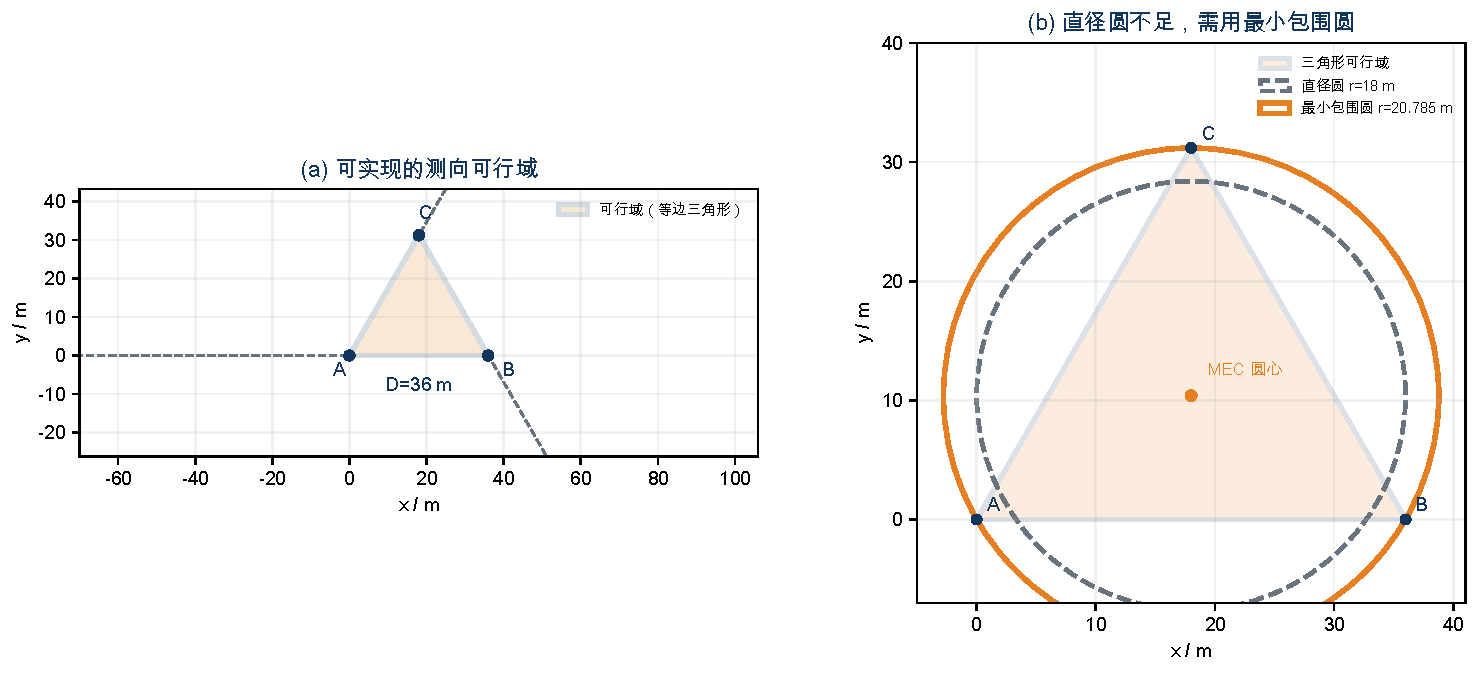
\includegraphics[width=\textwidth]{figures/geometry.pdf}
\caption{直径为36米的可实现三角形反例。任何半径18米的圆都无法覆盖三顶点；正确包围半径约20.785米。}
\end{figure}

\subsection{用最小包围圆直接连接定位与清除}
定义
\begin{equation}\label{eq:mec}
r_*(P)=\min_z\max_{p\in P}\norm{p-z},\qquad z_*(P)=\argmin_z\max_{p\in P}\norm{p-z}.
\end{equation}
圆盘是凸集，包含多边形所有顶点即包含整个多边形。最小包围圆由一个、两个或三个边界支持点确定，可用随机增量支持点算法求解\cite{welzl}。本文实现对近共线三点重算高精度行列式，并在最终半径上保留向外余量。

平面Jung界为
\begin{equation}\label{eq:jung}
\frac{D(P)}2\le r_*(P)\le\frac{D(P)}{\sqrt3}.
\end{equation}
两点支持时左端取等；三点支持时圆心在支持三角形内，三段圆心角中最大的一段至少$120^\circ$，对应弦长至少$\sqrt3r_*$，得到右端。等边三角形取右端等号。因此：
\begin{itemize}
\item $r_*(P)\le20$是存在一次保证清除点的充要几何条件；执行点取$z_*(P)$。
\item 仅使用直径时，$D(P)\le20\sqrt3$是充分条件，$D(P)>40$则必不可能一次保证覆盖。
\item $20\sqrt3<D(P)\le40$时必须进一步算包围圆，不能凭直径直接清除。
\end{itemize}

\subsection{在线使用的保守多边形}
在问题三、四中，每次有效示向度还说明$\norm{g-s_i}\le1500$。为保持纯线性裁剪，可使用安全松弛
\begin{equation}
u(\theta_i)^\mathsf T(g-s_i)\le1500.
\end{equation}
这不是把接收半径错误设为1500，而是利用其已知上界。若初始外切多边形为$A_{180}$，则维护
\begin{equation}\label{eq:poly}
\poly_c=A_{180}\cap\bigcap_{i\in I_c}\left(W_i\cap\{g:u(\theta_i)^\mathsf T(g-s_i)\le1500\}\right).
\end{equation}
真实源初始在$A_{180}$内，每条新增约束也包含它，故归纳得到$g_c\in\poly_c$。一次观测裁剪四个半平面，$m$次观测最多形成$180+4m$条边，复杂度$O(180m+m^2)$。空交集是需要定位原因的异常，而不是允许重置状态的信号。

\section{问题二：第二检测点的安全候选区域与选点策略}
\subsection{单次测向为什么没有唯一最优第二点}
只有角度而没有距离时，目标位于长而窄的扇形中。若第二点沿首次示向方向移动，两条示向线可能几乎平行或反平行，径向误差难以压缩。若仅为了接近$90^\circ$交会而绕行很远，则会增加移动时间，未必有利于题目总目标。

令$r_i=\norm{g-s_i}$、$u_i=(g-s_i)/r_i$、$n_i=(-u_{iy},u_{ix})$。对小误差线性化，有
\begin{equation}\label{eq:strip}
|n_i^\mathsf T\delta g|\le\alpha r_i.
\end{equation}
两条误差带交形成的平行四边形面积近似为
\begin{equation}\label{eq:area}
A\approx\frac{4\alpha^2r_1r_2}{|\sin\beta|},
\end{equation}
其中$\beta$为两条真实视线夹角，$\alpha$以弧度计。固定距离时，$90^\circ$交会最有利；距离也变化时，应同时考虑缩短$r_2$、避免共线及移动代价。该式是局部解释，不能代替精确楔形裁剪。

若额外采用独立高斯角误差的辅助似然，才可写出Fisher信息$J=\sigma^{-2}\sum_i n_in_i^\mathsf T/r_i^2$及$\det J=\sin^2\beta/(\sigma^4r_1^2r_2^2)$。没有这种似然假设时，这至多是加权最小二乘的局部信息代理，不能当成题目提供的真实误差统计模型。最终安全性仍由式\eqref{eq:poly}保证。

\subsection{利用首次已接收事实推导三圆交}
取第一次检测点$S_1$为局部原点，首次读数方向为$u$，法向为$n$，第二点写为
\begin{equation}S_2=S_1+tu+bn.\end{equation}
若可能真实距离为$r$，首次已经接收说明
\begin{equation}R\ge\max(1000,r),\end{equation}
而不仅仅是$R\ge1000$。设$F_1$为当前全部可能源位置，则保证全向源在第二点仍有信号或返回近源的精确鲁棒条件为
\begin{equation}\label{eq:receive}
S_2\in\bigcap_{g\in F_1} B\bigl(g,\max(1000,\norm{g-S_1})\bigr).
\end{equation}
用完整扇形$r\in[0,1500]$、角差$\varphi\in[-\alpha,\alpha]$覆盖真实$F_1$，可得闭式充分候选域。

\begin{theorem}[三圆交接收保证]\label{thm:lens}
令$u_\pm=u(\theta_1\pm\alpha)$。以下候选域内的任一点，对整个放宽扇形都能保证全向接收：
\begin{equation}\label{eq:lens}
\mathcal C=S_1+\bigl[B(0,1000)\cap B(1000u_-,1000)\cap B(1000u_+,1000)\bigr].
\end{equation}
对这一完整扇形，式\eqref{eq:lens}也恰好是式\eqref{eq:receive}的交集；若再利用圆域等更强先验，它可能不是最大的安全候选域。
\end{theorem}
\begin{proof}
写$q=S_2-S_1$。必要性由$r=0$和$r=1000,\varphi=\pm\alpha$给出。反之，两端圆约束意味着$q^\mathsf Tu_\pm\ge\norm q^2/2000\ge0$。小于$180^\circ$的中间短弧上，$q^\mathsf Tu_\varphi$的最小值在端点，因此对所有允许角度都满足同样下界。若$r\le1000$，距离$\norm{q-ru_\varphi}$关于$r$是凸函数，两端$r=0,1000$均不超过1000，内部也不超过1000；若$r\ge1000$，
\[
\norm{q-ru_\varphi}^2-r^2=\norm q^2-2r q^\mathsf Tu_\varphi\le0.
\]
故距离不超过$\max(1000,r)$，由首次接收所隐含的半径下界即可保证可检测。
\end{proof}

\subsection{显式候选区域与可执行搜索}
在$(t,b)$局部坐标中，三圆交等价于
\begin{equation}\label{eq:lenscoord}
\left\{\begin{aligned}
t^2+b^2&\le1000^2,\\
(t-1000\cos\alpha)^2+(b-1000\sin\alpha)^2&\le1000^2,\\
(t-1000\cos\alpha)^2+(b+1000\sin\alpha)^2&\le1000^2.
\end{aligned}\right.
\end{equation}
令
\begin{equation}
b_{\max}(t)=\min\left\{\sqrt{1000^2-t^2},\sqrt{1000^2-(t-1000\cos\alpha)^2}-1000\sin\alpha\right\}.
\end{equation}
根号有定义且$b_{\max}\ge0$时，$0<t<1000$、$0<|b|\le b_{\max}(t)$形成首次方位两侧的横向候选区。排除$b=0$用于避免把共线点作为唯一方案，而非禁止为了接近目标沿轴行进。

程序按下式构造42个候选：
\begin{equation}
\begin{aligned}
t&\in\{125,250,375,500,625,750,875\}\ \text{米},\\
b&=\pm\kappa b_{\max}(t),\qquad \kappa\in\{1/4,1/2,3/4\}.
\end{aligned}
\end{equation}
对每个候选模拟允许的第二读数，计算新多边形最小包围圆；优先选择采样最坏半径较小的点，可再以本步移动和检测代价打破并列。所有这些点的接收安全性来自定理\ref{thm:lens}，不是来自采样。

\begin{figure}[H]\centering
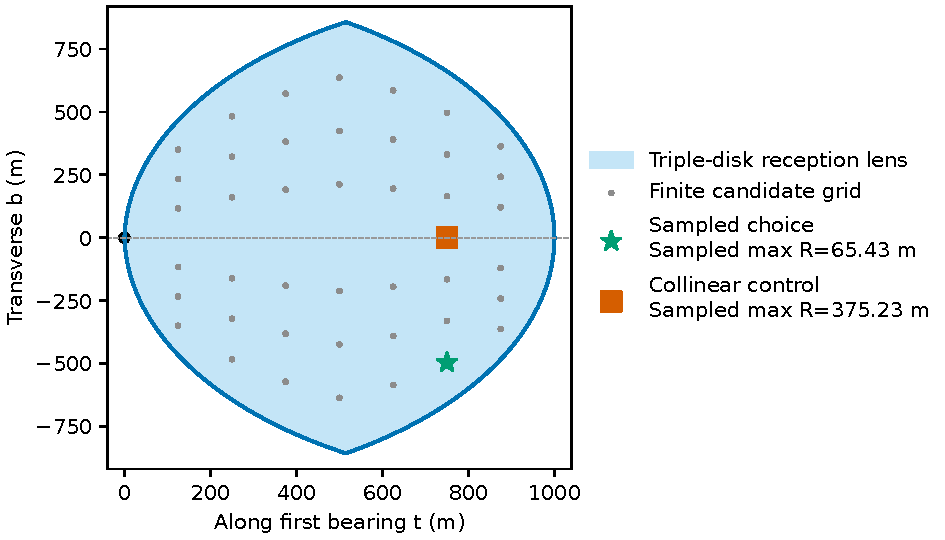
\includegraphics[width=\textwidth]{figures/q2_lens.pdf}
\caption{第二点的三圆交候选区域。横向基线改善交会条件，但候选排序仍需兼顾移动耗时和未知径向距离。}
\end{figure}

在$S_1=(0,0),\theta_1=0$的归一化示例中，取60个径向位置、3个首次真实角差和3个第二次测向误差进行比较。程序得到采样最佳几何候选约为$(750,-496.078)$米，采样最坏包围半径约65.426米；共线对照$(750,0)$的对应值约375.231米。两者本步耗时分别约184.844秒和155秒。这说明增加约29.844秒移动检测成本可显著改善此例的径向辨识，但第二次测向后仍未必能一次清除。

该示例是候选域与评分算法的演示，不是题目给定正式案例，也不是连续最坏情形或总时间的全局最优解。二维方位误差的连续极值、未知距离分布及后续代价若未严格处理，不能将网格最小值写成“最优定位策略”。

\section{局部定位：快速测向与有限光学兜底}
\subsection{正常测向路径}
针对已确认存在的频道，反复计算$(z_*,r_*)$：
\begin{enumerate}
\item 当前点到全部多边形顶点距离都不超过19.9米时，直接原地保证清除；否则若$r_*\le19.9$，移动到$z_*$保证清除。
\item 若$r_*\le38$米，可先在$z_*$进行一次光学尝试。失败仅花3秒且记录为失败，不将其写成保证成功；随后使用全区域覆盖，避免为一个很小区域继续绕远测向。
\item 设最近一次正测向点为$s^+$，从$s^+$指向$z_*$的单位方向为$u$、法向为$n$，候选测点取$z_*\pm\delta n$，其中$\delta=\min(120,\max(25,0.22r_*))$米。优先较近且未重复正读数的位置。
\item 对实际返回的正示向度继续裁剪；\texttt{near}立即原地清除。每次局部定位最多使用6个新测向点，随后转入光学覆盖。
\end{enumerate}

这里的25、120、38、0.22和6是公开的工程策略参数，而非从题面推导的自然常数。它们影响效率，不影响后备覆盖的正确性。问题二给出的是保证全向接收的完整候选域；本节采用更直接的中心横向点以降低重复评分开销，\textbf{没有声称每个在线测点都属于三圆交或总能保持信号}，而是对失去信号设置了可靠处理。

\subsection{定向源丢信号后的有限恢复}
问题四中，新的点可能越过发射半平面的边界。设失败点相对最近正测向点的分解为$q^--s^+=a u+b n$，下一点建议取
\begin{equation}\label{eq:recovery}
q^{\rm next}=s^++\tfrac12(a u-b n).
\end{equation}
其含义是向已知能接收的位置退回，同时尝试另一侧。新正测向可收缩位置多边形并更新$s^+$；持续无信号则继续有限恢复，直到达到6次测向上限。

式\eqref{eq:recovery}只是利用正负观测进行选点的启发式，不据此删除任何可能源位置，也不假称一定重获信号。它的价值通过最低接收半径、朝外边界源和聚集源的消融实验评价；最终清除保证不依赖恢复成功。

\subsection{覆盖整个可行多边形，而非只覆盖顶点}
若无法继续有效测向，取多边形的一条直径方向为局部$x$轴，将$P$包含在投影矩形中。把矩形划分为边长分别不超过$\sqrt2\rho_{\rm opt}$的网格单元，在每个单元中心放置半径$\rho_{\rm opt}=19.9$米的光学清除圆盘。每个单元半对角线不超过$\rho_{\rm opt}$，故
\begin{equation}\label{eq:optcover}
P\subseteq\bigcup_{j=1}^{J}B(q_j,\rho_{\rm opt}).
\end{equation}
注意多个圆盘的并集一般不凸，覆盖所有顶点并不能推出覆盖内部；本文覆盖的是整个外包矩形，因此不存在内部孔洞。

按蛇形访问这些中心，可把起点循环移动到距离当前位置最近的中心；这样最多增加一次跨行程的长跳。每个失败清除只排除该清除圆盘里的目标可能性，不把剩余非凸集合强行当成一个更小的凸多边形。实际源始终在$P$内，故尝试完全部中心之前必有一次成功，随后立即停止该频道的搜索。

\subsection{默认配置的有限动作与虚拟时间上界}
\label{sec:default-finite-bound}
本节覆盖最终\texttt{field}、官方演练所用原\texttt{refined}及历史\texttt{enhanced}策略：问题三均用原点及半径1200的六点环，问题四前两者用25点双环、后者用990米31点三角格。联合调度只重排任务，已知频道筛选不增加补测义务；均保留每局部任务至多6次固定测向和原矩形光学后备。\texttt{field}每任务另允许至多一次原地预检测，问题三负观测的保守凸外包不扩大原域、保证清除的安全接近不增加当次接入距离。假定接口正常、误差模型成立且无现实时间中断。以下沿用较大的31点范数与次数界，仅为新预检测增加检测预算；不涵盖条带光学或自适应候选。此界不声称紧或最优，距离单位均为米。

\paragraph{可行域尺寸与216单元证书。}
记真源为$g$，最近正示向点为$s$，$\alpha=1.005^\circ$。示向轴坐标满足$0\le x\le1500$、$|y|\le x\tan\alpha$。计入显式外扩，令$\varepsilon=10^{-7}$，取
\[
 X=1500+2\varepsilon,\qquad
 W=2\bigl((1500+\varepsilon)\tan\alpha+\varepsilon/\cos\alpha\bigr).
\]
于是纵向长度至多$X$，横向宽度至多$W<53$，$\sqrt{X^2+W^2}<1501$。最小包围圆圆心$z\in P$，故$\operatorname{diam}(P)<1501$且$\|z-s\|<1501$。正测点范数至多3300、初始外切多边形范数小于1801，使相关\texttt{\_padding}为$10^{-9}<\varepsilon$；此为几何与显式外扩的解析界，不是全部浮点运算的形式化认证。

单点域直接用一圆覆盖。否则设直径端点差为$(a,b)$、$d=\sqrt{a^2+b^2}>0$。任意点差满足$|\Delta x|\le d$、$|\Delta y|\le W$、$|b|\le W$，故直径法向投影差$|-b\Delta x+a\Delta y|/d\le2W$。计入投影外扩，直径对齐矩形仍长小于1501、宽小于106，对角线小于1505。令$h_-=\sqrt2(19.9-8\varepsilon)$，不大于代码单元边长上限，则
\begin{equation}
 J\le\left\lceil\frac{1501}{h_-}\right\rceil
       \left\lceil\frac{106}{h_-}\right\rceil
   =54\times4=216
\end{equation}
个半径19.9的圆盘覆盖整个矩形。蛇形相邻中心距至多$\sqrt2\,19.9$，循环移位至多增加一条矩形内跳跃，故
\begin{equation}
 L_{\rm snake}\le(216-1)\sqrt2\,19.9+\sqrt{1501^2+106^2}<7570.
\end{equation}
每个覆盖中心$q_{\rm opt}$与$g$均在同一矩形中，故$\|q_{\rm opt}-g\|<1505$。

\paragraph{恢复点必须以最近正测点为中心估计。}
固定候选$q_0=z\pm\delta n$满足$n\perp(z-s)$、$\delta\le120$，因此$\|q_0-s\|\le A:=\sqrt{1501^2+120^2}<1506$。
在获得新正示向前，所有恢复仍使用同一个$s$。设$R_k$为相应轴向反射，则
\[
 q_{k+1}-s=\tfrac12R_k(q_k-s),\qquad
 \|q_{k+1}-s\|=\tfrac12\|q_k-s\|.
\]
反射只保持到$s$的距离，不能把失败点的源距与1500取平均。故连续恢复有$\|q_k-s\|\le2^{-k}A$；新正示向更新$s$后重用首点界。由$\|s-g\|\le1500$，全部局部测向点满足
\begin{equation}
 \|q-g\|\le B:=1500+A<3006,\qquad
 \|q\|\le1800+B<4806.
\end{equation}
圆心源距小于1501，覆盖中心源距小于1505，两者范数亦小于4806。测向间连线至多$2B<6020$；额外圆心清除接入至多$B+1501<4520$；光学接入至多$B+1505<4520$，若紧接圆心试清则至多$1501+1505<4520$。

\paragraph{任务进出、动作计数与总界。}
每任务至多6次固定测向，\texttt{field}在进入该过程前另可执行一次原地预检测；各提前返回分支均成功清除或转入有限光学覆盖。真源在覆盖域内，故每个正常完成任务必清除一新源，任务数至多16。成功终点距该源至多20、范数至多1820；原地预检测、共享补测及其\texttt{near}清除不移动。这处理了从\emph{另一源清除点}进入下一任务的情形。

骨架点范数至多$990\sqrt7<2620$。集成策略整次骨架扫描不插入局部移动，故至多31次骨架抵达，出发于原点、骨架或成功清除点，每段小于5240。任务首个需移动的动作由范数至多2620的任务外位置进入范数小于4806的局部点，入口小于7500；原地预检测不改变入口位置。此后至多5条测向连线、一次额外圆心清除移动（保证清除或小区域试清）、一次光学接入及一条蛇形，故
\begin{equation}
 L\le31\times5240+
 16\bigl(7500+5\times6020+4520+4520+7570\bigr).
 \label{eq:corrected-travel-bound}
\end{equation}
若首动作即圆心清除或光学首点，入口已支付该段，多余预算仅为放宽。任务至下一骨架的退出段已计入31次骨架抵达；无需返回原锚点。

骨架至多$31\times20$次测向；共享只在任务结束后调用，至多16次、每次至多16源；固定局部测向至多$16\times6$次。\texttt{field}原地预检测在六次之外，每任务至多一次，另加16次且不新增行程。放宽共享预算得到
\[
 M\le31\times20+16\times16+16\times6+16
 \le31\times20+31\times16+16\times6+16=1228.
\]
每源无信号后试清至多6次、小区域试清至多一次、覆盖至多216次，另留一次给非覆盖成功清除（骨架、共享、局部\texttt{near}或保证清除）；成功后不再处理，故$C\le16(216+6+1+1)=3584$。移动速度为5米/秒，测向含换频至多6秒，清除至多5秒，因而
\begin{equation}
 \begin{split}
 T&\le\frac{31\times5240+
 16(7500+5\times6020+4520+4520+7570)}5\\
 &\quad+1228\times6+3584\times5
 <100\times3600\ \mathrm{s}.
 \end{split}
\end{equation}
这是虚拟时间保守界，不是预期成绩或最优界；\texttt{refined}/\texttt{enhanced}没有新增预检测，仍可使用原$M\le1212$。\texttt{field}的任务重排及域缩小不改变其余范数、行程和光学次数预算，上界也不表示每个实例更快。现实20分钟限制须由客户端期限机制另行遵守。


网络故障可能耗尽现实时间，任何算法都不能对无限网络延迟保证20分钟内完成。客户端必须按真实剩余时间停止并报告未完成，不能将这类异常伪装成全清；本文尚未验证官方接口条件下的现实耗时。

\section{问题三：七点覆盖与观测驱动调度}
\subsection{七点发现骨架的解析构造}
取
\begin{equation}\label{eq:omni}
p_0=(0,0),\quad p_{k+1}=900\sqrt3\left(\cos\frac{k\pi}{3},\sin\frac{k\pi}{3}\right),\quad k=0,\ldots,5.
\end{equation}
环半径约1558.846米，而覆盖圆半径只需900米。

\begin{theorem}[全向七点不漏检]
$\disk\subseteq\bigcup_{k=0}^{6}B(p_k,900)$。因有效接收半径至少1000米，在每点检测全部未清除频道必能发现每个尚存的全向源。
\end{theorem}
\begin{proof}
若$r=\norm g\le900$，原点即可覆盖。若$900\le r\le1800$，存在一个环点与$g$的极角差不超过$30^\circ$，因此
\[
\norm{g-p_k}^2\le r^2+3\times900^2-3\times900r.
\]
右端是凸二次函数，在$[900,1800]$上的最大值取在端点，均等于$900^2$。圆周边界与环点夹角平分线同样包含在证明内。
\end{proof}

\subsection{每频道的完成证书}
为每个频道保留以下状态：已确认清除、已发现但未清除、尚未确定。逐频道记录实际检测过的骨架索引。若某未清除频道在全部七个点都返回无信号，则由覆盖定理可认证该频道无源；若曾经检测到源，则必须获得成功清除反馈，不能因后来无信号而把它当成无源。

因此正确停止条件是：20个频道各自都已清除或已获得完整覆盖的无源证书。另一个合法提前停止条件是已确认清除了16个不同频道，因为这达到题给总数上界。清除10个、长时间没有新源、已知目标队列为空均不足以停止。

全向无信号还可排除检测点1000米范围内的该频道源，但当前实现不把这种非凸位置减法强塞进凸多边形；它主要用无信号完成骨架证书。虽然可能多走一些路，解释与安全边界更清楚。

\subsection{三个可复现的调度层次}
\textbf{基线A（baseline）：}最近未访问骨架点依次扫描频道，一检测到源就离开骨架点完成该源定位清除，再返回继续剩余频道。它简单且有完整覆盖保证，但多源时往返多。

\textbf{策略B（batched）：}在同一骨架点先完成所有未清除频道的检测，合并维护已发现源。每步在访问新骨架与清除已知源之间做滚动决策。目标任务的分数取当前位置到其包围圆中心的距离；骨架任务分数取移动距离加$30n_u$，其中$n_u$为未清除频道数，30米等价于一次6秒检测切换的移动成本。该加项是扫描费用近似，不是精确价值函数。

\textbf{策略C（integrated）：}在B基础上，完成某源清除后利用已有停靠点为其他已知源补充测向。仅对区域尚大、可能处于1500米接收范围且当前位置未曾检测过的频道补测；历史位置按精确坐标去重，不把相距小于80米的不同地点误当作相同电磁环境。成功清除频道立即从后续扫描中剔除。

A到B的差异同时包括批量扫描和目标顺序选择，不能把其收益全叫作“共享观测收益”。B和C使用相同覆盖、局部定位和任务评分，只有补测共享开关不同，因此可用于共享机制消融。额外补测仍花5或6秒，个别案例可能增时，不能声称总是占优。

\section{问题四：任意发射方向下的31点覆盖}
\subsection{为什么不能沿用圆内全向搜索}
在圆域边界取一个向外发射的源，圆内绝大多数检测点都在其背面，即使距离远小于1000米也无信号。故“每个位置附近都有检测点”只保证全向覆盖，不保证定向覆盖。题目允许机器人提交圆域外坐标，必须利用这一条件。

\subsection{三角格和半平面凸包证书}
取$s=990$米，基向量$a=(s,0)$、$b=(s/2,\sqrt3s/2)$，保留
\begin{equation}\label{eq:lattice}
\mathcal V=\{ia+jb:i,j\in\mathbb Z,\ \norm{ia+jb}\le1800+s\}.
\end{equation}
任意$g\in\disk$位于一个边长$s$的基本闭等边三角形内。三个顶点都距$g$不超过$s$，范数不超过$1800+s$，故均在$\mathcal V$中。若$g=\sum_i\lambda_i v_i$，$\lambda_i\ge0$且和为1，则任意发射法向$n$满足
\begin{equation}\label{eq:hull}
\sum_i\lambda_i n^\mathsf T(v_i-g)=0.
\end{equation}
因而不可能所有正权重顶点都位于严格背面，至少一个点满足$n^\mathsf T(v_i-g)\ge0$并处于1000米以内，必有信号。源落在格边时利用含边界的发射规则；源正好位于圆域内的格点时，其六个邻点均被保留，任意朝向至少有一个非零邻点在前方。

格点范数平方为$s^2(i^2+ij+j^2)$。默认截断相当于$i^2+ij+j^2\le961/121<8$，出现的范数层只有$0,1,3,4,7$，点数分别为$1,6,6,6,12$，总计31；其中13点在目标圆内，18点在圆外。不能把这18点投影回圆域。

\begin{figure}[H]\centering
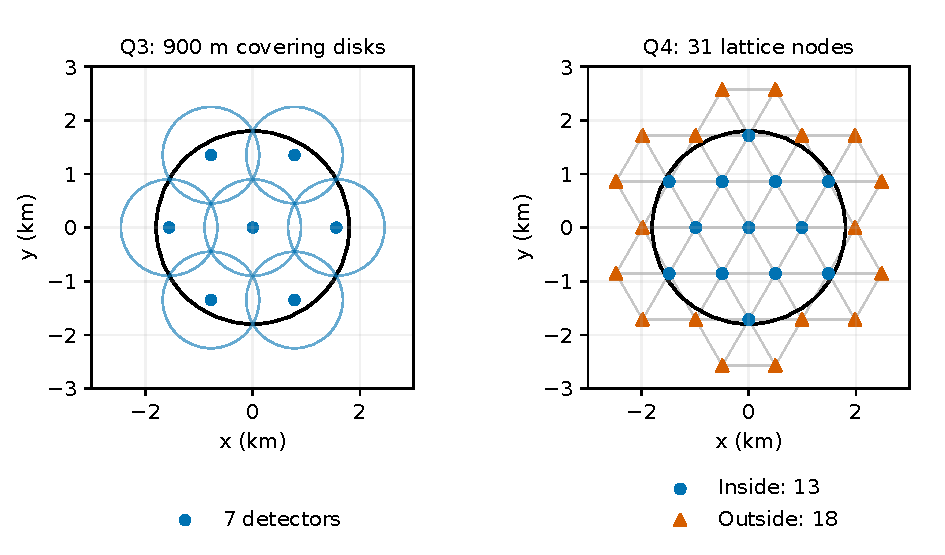
\includegraphics[width=\textwidth]{figures/coverage.pdf}
\caption{全向七点覆盖与定向31点覆盖。右图圆外格点是方向覆盖证书的一部分，而非可删除的冗余越界点。}
\end{figure}

\subsection{比“恰好在边界上”更强的数值余量}
默认点集还能给出严格正方向余量。给定$g,n$，令$h=g+5n$。包含$h$的基本三角形顶点满足$\norm{v-g}\le995$且$\norm v\le2795$。因$(2795/990)^2<8$且范数层是整数，其层号至多7，仍全在原31点中。它们的凸组合满足
\begin{equation}\sum_i\lambda_i n^\mathsf T(v_i-g)=5.\end{equation}
因此至少一个顶点正投影不小于5米、距离不大于995米。即使坐标产生不超过1米的欧氏扰动，该点仍在严格前方且距离不超过996米。这避免只依赖理想实数下的发射边界相等式。实际双精度坐标误差远小于这一余量。

\subsection{负观测的正确语义}
问题四中的\texttt{no\_signal}可能由无源、超出半径或处于背面导致，不能像全向情形那样直接删除1000米圆盘。若坚持更精细推断，应维护$(g,R,n)$的联合可行域：正观测要求距离及正半平面条件；当$\norm{s-g}\le1000$时，负观测可推出$n^\mathsf T(s-g)<0$，但位置与方向不可分离处理。

当前实现选择不增加这一高维状态维护，而以正测向多边形、有限失信号恢复与完整光学覆盖完成局部任务。这是主动保持保守性，不是忽略定向条件：31点发现定理和方向无关的光学清除正好给出了两个端点保障。

搜索调度、逐频道完成判据及16源上界提前停止均与问题三相同，只将七点骨架换为31点，并启用式\eqref{eq:recovery}。骨架检测最多$31\times20=620$次；这不包含局部检测，但已清除频道不再扫描。

\section{统一求解流程、下界与策略筛选}
\subsection{部分可观测状态机与证书不变量}
将机器狗搜索过程表示为部分可观测状态机。连续状态为位置$q_t$、各频道定位多边形和观测历史，离散状态为测向机当前频道、已接受动作日志及频道证书。记频道$c$的状态为
\[
Z_c(t)\in\{U,D,C\},
\]
其中$U$表示尚未发现，$D$表示已发现但尚未确认清除，$C$表示已确认清除；无源认证另由$\operatorname{Cert}_c=N$表示。全局状态为
\[
X_t=\left(q_t,k_t,\{Z_c(t),V_c(t),P_c(t)\}_{c=1}^{20},A_t\right),
\]
其中$k_t$是测向机频道，$V_c$是已完成的骨架检测点集合，$P_c$是正示向形成的保守多边形，$A_t$仅含已接受的请求及响应。
令$V$表示当前题型的完整骨架：问题三为$V_3=\{0,\ldots,6\}$，问题四为$V_4=\{0,\ldots,30\}$；证书中的$V$按当前问题取$V_3$或$V_4$。

隐藏真实状态$\xi_c$可能为空，也可能包含位置、接收半径和定向方向；程序绝不读取$\xi_c$。令$F_c(t)$为与该频道截至$t$时刻全部已接受响应相容的联合状态集合。我们的更新规则满足
\begin{equation}\label{eq:state-invariant}
\xi_c\in F_c(0)\Longrightarrow \xi_c\in F_c(t),
\qquad F_c(t+1)\subseteq F_c(t).
\end{equation}
正示向只加入真实误差楔形及安全距离帽；\texttt{no\_signal}在问题四中不单独删去位置圆盘；失败清除只记录失败位置。因而即便效率较低，式\eqref{eq:state-invariant}仍不被启发式路线破坏。

频道完成证书定义为
\begin{equation}\label{eq:certificate}
\operatorname{Cert}_c(t)=
\begin{cases}
C,&\text{收到该频道成功清除响应},\\
N,&Z_c(t)=U,\ V_c(t)=V,\ \text{且所有检测均为有效\texttt{no\_signal}},\\
U\text{或}D,&\text{其他情况}.
\end{cases}
\end{equation}
这里$D$状态一旦出现就不能被后续无信号改写为$N$。因为一个已知存在的源不会因改变检测点而消失，且问题三、四的覆盖证书分别保证全向源或任意方向定向源至少被检测一次，故
\[
\forall c,\quad \operatorname{Cert}_c\in\{C,N\}
\]
是安全停止条件；确认清除16个不同频道是利用题目上界的另一种安全停止条件。这个定义比“当前待处理队列为空”更强，也比依赖字典中是否存在某个轨迹更稳定。

动作状态还需满足协议原子性：只有响应完整且$\texttt{accepted=true}$时，才推进$X_t$；截断响应重试时保留原请求编号和请求字节；不确定动作禁止发送不同的新动作。若已接受动作到达虚拟时间上限，先保留该动作的观测结果，再检查已有证书；若证书未完成则返回“不完整超时”，绝不再发送$\texttt{/exit}$。这一点由\texttt{SessionTerminated}、\texttt{terminal\_reason}和独立终端回归脚本共同实现。

\subsection{正确性风险与时间代价分解}
将风险拆为发现、定位、清除和停止四类：
\[
R_D,\ R_L,\ R_C,\ R_S.
\]
对于解析保证范围，要求对每一个合法世界均有
\begin{equation}\label{eq:zero-risk}
R_D=R_L=R_C=R_S=0.
\end{equation}
覆盖点集和凸包半平面证书解决$R_D$，保守多边形和完整光学外包矩形解决$R_L$，接口返回\texttt{success}才更新清除状态解决$R_C$，式\eqref{eq:certificate}解决$R_S$。有限合成试验只能检查实现是否符合这些条件，不能把有限样本中的零失败率写成数学上的零风险。

总虚拟时间严格拆分为
\begin{equation}\label{eq:cost-decomposition}
T=T_{\rm move}+T_{\rm measure}+T_{\rm switch}+T_{\rm fail}+T_{\rm clear}
=\frac{L}{5}+5M+S+3F+5K.
\end{equation}
这一区分能够解释改进的作用：批量扫描主要减少$L$，共享停靠可能增加$M$但减少$L$，定向失信号恢复用少量移动和检测换取$F$下降，光学兜底增加失败清除次数但不依赖错误的负观测解释。只报告总时间而不拆分这些项，不能说明机制的真实贡献。

因此我们采用字典序决策：先保留证明域内的全清和逐频道证书，再最小化$T$，最后才考虑$M$和$L$。对没有完整证明的候选策略，只报告相对于安全基线的配对经验差
\begin{equation}\label{eq:regret}
\widehat{\operatorname{Reg}}(\widehat\pi;\pi_0)
=\frac1n\sum_{j=1}^n\left(\frac{T_j(\widehat\pi)}{N_j}-\frac{T_j(\pi_0)}{N_j}\right),
\end{equation}
其中$n$是配对世界数，$\widehat\pi$为候选策略，$\pi_0$为安全对照。还须报告未清除数、证书状态与分项成本，不能把负的经验差解释为全局最短路。

\subsection{覆盖半径下界和构型最小性边界}
\label{sec:cover-lower}
对区域$\Omega$和有限检测点集$Q$定义覆盖半径
\begin{equation}\label{eq:cover-radius}
\rho_{\rm cov}(Q;\Omega)=\max_{x\in\Omega}\min_{q\in Q}\|x-q\|.
\end{equation}
完整覆盖的充要条件是$\rho_{\rm cov}(Q;\Omega)\le r$。若$n$个半径$r$圆盘覆盖面积为$|\Omega|$的区域，则有面积下界
\begin{equation}\label{eq:area-lower}
r\ge\sqrt{\frac{|\Omega|}{n\pi}}.
\end{equation}
该下界忽略重叠和边界效应，通常不紧；因此本文不把31点或七点直接称为任意点集中的全局最少点方案。

但是，对问题三采用的保守覆盖半径$900=1800/2$，单个检测点位于距圆心$d$处时，其对目标圆周的最大覆盖半角不超过
\[
\alpha_{\max}=\arcsin(900/1800)=30^\circ.
\]
六个半径900米圆盘要覆盖整条圆周，必须六个点均达到最大60度覆盖弧并恰好分割圆周；这迫使它们位于半径$900\sqrt3$的规则环上，但此时原点距任一环点为1558.846米，原点未被覆盖。因此，在该保守半径和圆心加环的证明框架内，七点是精确下界；这不等价于物理半径固定为1000米时任意六点构型都不可能。

对于问题四，31点是半径2790米截断下的完整三角格集合：
\[
i^2+ij+j^2\le(2790/990)^2=961/121<8.
\]
其壳层$0,1,3,4,7$的点数为$1,6,6,6,12$。对当前三角格的方向无关证书，每个点都是不可随意删除的：在其对边中点向顶点方向略微移动源位置，顶点是唯一同时满足正投影和1000米距离的格点。该结论只证明“当前格点证书的不可删性”，不宣称所有可能的31点外部布局都是全局最优。

\subsection{算法流程、复杂度与可复现性}
主算法可概括为：
\begin{enumerate}
\item 初始化目标圆域外切多边形、骨架义务$V$、频道状态$Z_c=U$及当前位置；
\item 在当前骨架点按频道顺序逐一检测。返回\texttt{no\_signal}\allowbreak{}只记录义务；返回\texttt{direction}\allowbreak{}则以真实读数裁剪$P_c$；返回\texttt{near}\allowbreak{}立即调用清除；
\item 在所有骨架义务完成前，依据当前位置、未清除频道数和已有$P_c$的MEC中心选择“继续覆盖”或“定位已有目标”；
\item 对已发现频道最多进行6次局部测向。问题四丢失信号时执行有限退回反侧策略；任何时候只用实际正示向更新$P_c$；
\item 若MEC不能保证一次清除，使用覆盖整个外包矩形的19.9米光学圆盘蛇形路径；清除成功即将该频道置为$C$；
\item 全部频道均为$C$或$N$，或已确认16次成功清除时停止；遇到真实截止则输出终端原因，不伪造全清。
\end{enumerate}
本文最终增强策略的有限虚拟时间上界见第\ref{sec:default-finite-bound}节。该证明按最近正测点周围的反射半缩递推，分别支付任务入口、最多五条测点连线、小区域试清、光学接入和蛇形覆盖；没有将关于测点的反射误当成关于真实源的等距变换。增强只收缩Q3骨架并滚动重排Q4骨架，不改变发现证书；区间自适应测点候选不纳入默认上界。

\subsection{有对照的改进筛选}
\begin{table}[H]\centering\small
\caption{未采用候选的配对对照；“节省”定义为对照时间减候选时间，负值表示候选增时}\label{tab:candidate-negative}
\begin{tabular}{@{}>{\raggedright\arraybackslash}p{0.8cm}@{\hspace{0.14cm}}>{\raggedright\arraybackslash}p{2.4cm}@{\hspace{0.14cm}}>{\raggedleft\arraybackslash}p{2.1cm}@{\hspace{0.14cm}}>{\raggedleft\arraybackslash}p{2.1cm}@{\hspace{0.14cm}}>{\raggedleft\arraybackslash}p{2.1cm}@{\hspace{0.14cm}}>{\raggedleft\arraybackslash}p{1.9cm}@{\hspace{0.14cm}}>{\raggedleft\arraybackslash}p{2.6cm}@{}}
\toprule
问题 & 候选 & 对照/s & 候选/s & 节省/s & 更快/对 & 全清数\newline 对照/候选 \\
\midrule
Q3 & 静态2-opt & 316.38 & 339.46 & -23.07 & 33/200 & 200/200 \\
Q3 & 自适应探测 & 311.80 & 337.36 & -25.56 & 0/200 & 200/200 \\
Q4 & 静态2-opt & 822.26 & 876.66 & -54.40 & 40/200 & 200/200 \\
Q4 & 自适应探测 & 805.77 & 810.69 & -4.92 & 70/200 & 200/200 \\
\bottomrule
\end{tabular}

\end{table}
静态2-opt在出发前优化的路线不能预见局部清除后的实际位置；自适应测点评分则只优化正示向后几何不确定性的上界，并不是完整任务的价值函数。它可以减少Q4失败清除次数，却付出额外测向、移动和计算。表中结果不否定主动测向理论，只否定本次有限候选及权重配置的默认准入。

这两个负结果同样重要：模型升级的准入标准不是“公式更复杂”或“某个子指标更好”，而是相同证书下完整$T/N$具有稳定收益。最终策略仍采用简单固定偏移、问题四有限恢复和完整光学兜底，所有更复杂候选均不能绕过覆盖义务。

\subsection{敏感性、压力测试与可证范围}
对参数$\theta$，在固定种子和停止规则下报告
\[
S_Y(\theta)=
\frac{[Y(\theta)-Y(\theta_0)]/Y(\theta_0)}
{[\theta-\theta_0]/\theta_0},
\]
其中$Y$可取$T/N$、检测次数、失败清除次数或回退比例；若基准为零则使用绝对差。已有实验改变横向偏移尺度$0.12,0.22,0.40$以及三角格距$900,950,990$米，并在最小接收半径、朝外边界源、聚集源和三种固定误差场下检查。结果只支持声明的合成分布，不外推为官方世界的概率结论。

最终报告同时保存均值、中位数、最近秩$p_{90}$、最坏值、距离、测量次数、切换次数、失败清除次数和全清计数。对配对世界使用式\eqref{eq:regret}而非合并所有源的总时间比值；这样源数不同造成的尺度差异不会被误认为策略收益。

\section{有证据的搜索增强：环收缩与滚动路径}
\label{sec:enhancement}
\subsection{优化几何，而非减少证明义务}
原七点骨架的900米覆盖保证留有100米接收余量，但这一余量不必全部保留。机器狗的移动速度仅为5米/秒，约1559米的骨架环会形成较长的空频道排查路径；可在仍小于1000米的覆盖半径内，把检测环向圆心收缩。该改变没有减少七个检测位置，也没有推测某频道不存在，而是为每个新位置重新给出完整覆盖证书。

取$R=1800$，原点加六个角间隔$60^\circ$的环点，环半径为$d$。源的极径为$r$，选择角差不超过$30^\circ$的环点，则在该方向最坏角度处，到最近检测点的距离为
\begin{equation}\label{eq:ring-envelope}
 f_d(r)=\min\left\{r,\sqrt{r^2+d^2-\sqrt3dr}\right\}.
\end{equation}
两项相等时$r=d/\sqrt3$；交点之前原点更近，之后环点更近。在$[d/\sqrt3,R]$上，根号内是凸二次函数，所以最大值在端点取得。只要$d/\sqrt3\le R$，整个圆域的精确覆盖半径为
\begin{equation}\label{eq:contracted-cover}
 \rho_{\rm ring}(d)=\max\left\{\frac d{\sqrt3},
 \sqrt{R^2+d^2-\sqrt3Rd}\right\}.
\end{equation}
这不仅给出上界：相邻环点的角平分线在$r=d/\sqrt3$及$r=R$处分别达到两项，因此是精确值，而不是网格采样估计。

要求$\rho_{\rm ring}(d)\le q$，其中$q$是选用的安全接收半径，得到
\begin{equation}
 d\le\sqrt3q,\quad
 \frac{\sqrt3R-\sqrt{4q^2-R^2}}2\le d\le
 \frac{\sqrt3R+\sqrt{4q^2-R^2}}2.
\end{equation}
当$q=900$时只有原构型的$d=900\sqrt3$；当允许$q$向物理下界1000靠近时，可选更小的$d$。本文不取恰好触及1000米的极限值，而固定$d=1200$米，计算得到
\[
 \rho_{\rm ring}(1200)=968.901572\ \mathrm m,
 \qquad 1000-\rho_{\rm ring}(1200)=31.098428\ \mathrm m.
\]
该余量远大于双精度和坐标舍入误差，也允许进行明确的覆盖灵敏度分析。若检测中心位置扰动不超过$\eta$米，三角不等式使覆盖半径至多增加$\eta$；故在$\eta<31.09$米时仍可保持物理距离覆盖。这不是题目要求的定位误差容许范围，而是布点构型的稳定性结论。

\begin{figure}[H]\centering
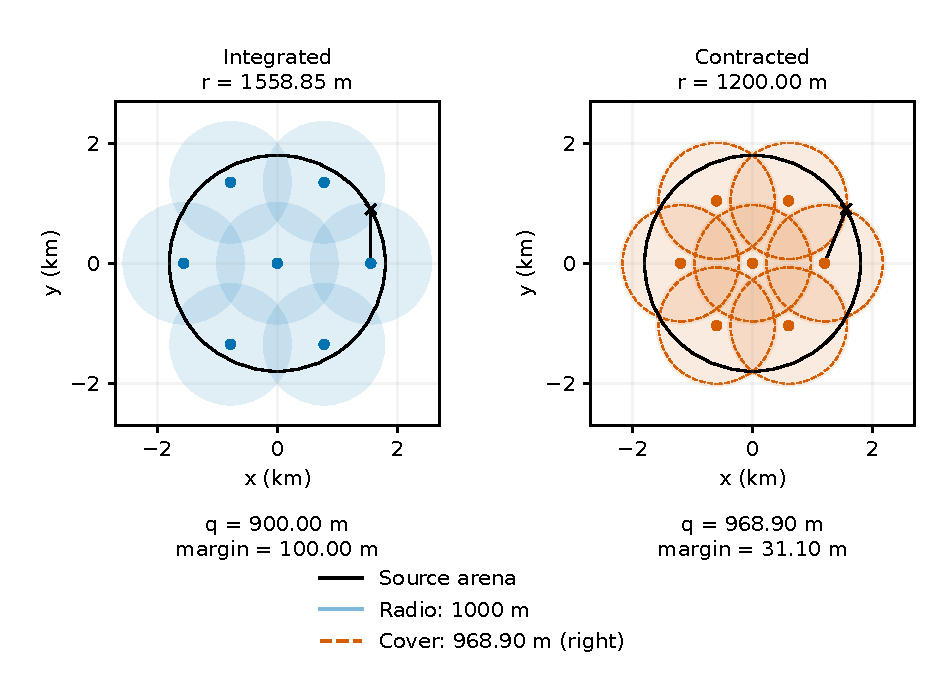
\includegraphics[width=\textwidth]{figures/enhancement_geometry.pdf}
\caption{七点覆盖的余量--行程权衡：1200米收缩环保持完整接收覆盖，不删去任何频道的检测义务。}
\end{figure}

\subsection{环半径的行程下界与候选筛选}
\label{sec:ring-sweep}
覆盖半径最小并不等价于任务时间最小。对原点与六个正六边形环点，若只考虑从原点出发、访问全部六个环点且不要求返回的骨架路径，则其精确最短长度为
\begin{equation}\label{eq:ring-tour}
L_{\rm skeleton}^{\min}(d)=6d.
\end{equation}
证明很直接：起点到第一个环点的距离为$d$，其后五条环点间连线的长度均不小于相邻点间距$d$，故总长至少$6d$；沿圆周依次访问恰好达到该下界。这个结论不含局部定位支线，也不适用于提前确认16源后省略剩余点的轨迹，但清楚解释了环收缩为何能减少\emph{骨架层}的移动成本。

在本文支持的区间$1200\le d\le900\sqrt3$上，式\eqref{eq:contracted-cover}由边界项控制，且
\[
\rho_{\rm ring}'(d)=\frac{d-\sqrt3R/2}{\sqrt{R^2+d^2-\sqrt3Rd}}\le0,
\qquad (L_{\rm skeleton}^{\min})'(d)=6.
\]
因此扩大检测环会改善最坏接收余量，却同时提高完整骨架行程下界；两者构成可解释的权衡，而非某一个指标越小越好。相较原半径，$d=1200$把纯骨架下界由$9353.07$米降到$7200$米，但完整任务仍可能因发现顺序与定位支线改变而增时，不能把这一下界差额直接当作实际节省。

为避免只比较两个半径就把1200米称为最优，本轮在既有开发种子1000000至1000149上比较8个候选半径，保持其余策略不变。表\ref{tab:ring-sweep}给出150个世界的开发均值；1200米胜出，1250米为次优。早期扩展比较曾复用1100000组数据，本表改用未参与此前筛选的2300000至2300499进行最终确认，冻结候选后不再调参。保存的2200次执行包括$8\times150$次开发运行与$2\times500$次新世界配对运行，不是2200个独立世界。
\begin{table}[H]\centering\small
\caption{Q3安全环半径筛选；时间单位为秒/源，破折号表示未进入样本外复核}\label{tab:ring-sweep}
\begin{tabular}{@{}>{\raggedleft\arraybackslash}p{1.5cm}@{\hspace{0.14cm}}>{\raggedleft\arraybackslash}p{2.2cm}@{\hspace{0.14cm}}>{\raggedleft\arraybackslash}p{2.0cm}@{\hspace{0.14cm}}>{\raggedleft\arraybackslash}p{2.1cm}@{\hspace{0.14cm}}>{\raggedleft\arraybackslash}p{2.6cm}@{\hspace{0.14cm}}>{\raggedright\arraybackslash}p{1.0cm}@{}}
\toprule
环半径/m & 解析覆盖/m & 开发T/N & 新样本T/N & 相对对照节省/s & 选择 \\
\midrule
1200 & 968.90 & 272.97 & 272.71 & 2.38 & 保留 \\
1250 & 951.52 & 274.88 & 275.09 & -- & 次优 \\
1300 & 936.48 & 277.58 & -- & -- &  \\
1350 & 923.91 & 281.27 & -- & -- &  \\
1400 & 913.91 & 286.18 & -- & -- &  \\
1450 & 906.56 & 293.27 & -- & -- &  \\
1500 & 901.92 & 298.08 & -- & -- &  \\
1550 & 900.04 & 305.55 & -- & -- &  \\
\bottomrule
\end{tabular}

\end{table}
1200米与1250米在500个新检验世界均全清；前者平均为\RingSelectedTime{}秒/源，后者为\RingControlTime{}秒/源。配对节省均值为\RingSaving{}秒/源，其近似95\%置信区间为$[\RingLowerCI,\RingUpperCI]$，\RingFaster/500个世界更快。故保留1200米作为当前默认，不引入新策略分支。此结论仅针对声明的候选集与合成分布，不声称连续半径、所有源分布或全部在线策略中的全局最优。

\subsection{从静态2-opt改为剩余任务的滚动重排}
固定骨架路线的静态2-opt只能减少骨架间纯移动，不能预知局部定位支线结束后机器狗在哪里。因此本文改为每次准备选择骨架任务时，从\emph{已接受动作确定的当前位置}出发，在未完成骨架点集合上重新建立最近邻开放路径，再做2-opt交换；只执行新的第一个骨架点，下一决策时重新规划。

设当前路径包含边$(a,b)$和$(c,d)$，交换区间方向可使其变为$(a,c)$和$(b,d)$，路径变化为
\begin{equation}\label{eq:two-opt-delta}
 \Delta L=\|a-c\|+\|b-d\|-\|a-b\|-\|c-d\|.
\end{equation}
仅当$\Delta L<0$且超过数值容差才接受。若区间到达开放路径终点，不计不存在的终端边。交换只反转索引子序列，故点集和逐频道义务不变；算法不允许因路程较远而删除圆外点。一次扫描$O(n^2)$个交换，严格下降在有限排列集合内终止。本文只给出每次2-opt扫描的解析复杂度；实验结果未单独记录其CPU时间或总扫描次数。

这一滚动方案的安全性与时间最优性必须分开：安全性仍由完整骨架和光学后备证明，2-opt仅是当次余程的局部搜索。下一次测向发现新源后，未来真实路线可能不同；因此每次的短路不保证每个世界总时间都缩短。Q3收缩环后仅采用最近点调度，因为开发样本中叠加滚动优化的收益很小；Q4采用滚动余点排序，因为开发比较显示其能减少实际长距离骨架路程。
\subsection{覆盖点数的下界与格点不可删性}
\begingroup\sloppy
Q3的900米覆盖构造和边界弧下界见式\eqref{eq:omni}及第\ref{sec:cover-lower}节；它们共同给出该保守半径下的精确七点结论，不是1000米物理接收下界下任意布局的全局最优性。

Q4的31点结论同样只针对当前$990$米三角格。逐点见证脚本在每个格点附近构造唯一可接收的定向源，因此删除当前集合中的任一点会破坏该证书；这不是对任意替代布局的全局点数下界。
再考察圆周上的径向外发射源。探测点范数为$d$、极角差为$\phi$时，前向条件为$d\cos\phi\ge R$；接收还要求$d^2+R^2-2dR\cos\phi\le q^2$。$d<R$或$d>R+q$均不可能接收，故单点最大覆盖角半宽为
\begin{equation}\label{eq:boundary-angle-bound}
\alpha_4=\max_{R\le d\le R+q}\arccos\!\left(\max\left\{\frac R d,\frac{d^2+R^2-q^2}{2dR}\right\}\right)=\arctan\frac qR.
\end{equation}
第一项随$d$递减，第二项在$d\ge R$递增，交点$d=\sqrt{R^2+q^2}$给出等号。$q=1000,R=1800$时，$\alpha_4=0.50710$弧度，故至少需要$\lceil\pi/\alpha_4\rceil=7$个圆外探测位置。该特殊边界下界与当前31点不可删性不同，不能推出31点全局最少。
\begin{table}[H]\centering\small
\caption{覆盖下界及当前固定集合的不可删性证据}\label{tab:coverage-limits}
\begin{tabular}{@{}>{\raggedright\arraybackslash}p{4.1cm}@{\hspace{0.14cm}}>{\raggedleft\arraybackslash}p{2.0cm}@{\hspace{0.14cm}}>{\raggedright\arraybackslash}p{8.7cm}@{}}
\toprule
Statement & Value & Interpretation \\
\midrule
Q3 q=900 lower bound & 7 & six boundary arcs at equality; origin uncovered \\
Q3 fixed seven-set at q=1000 & 7 & five ring arcs leave a boundary gap \\
Q4 outer-boundary lower bound & 7 & arbitrary placements; outer detectors only \\
Q4 current lattice witnesses & 31 & target d=856.365--856.365 m \\
Q4 nearest other lattice point & 495.001 m & every witness remains outside near threshold \\
\bottomrule
\end{tabular}

\end{table}
\endgroup

\subsection{隔离开发和检验的数据分工}
环收缩和滚动路线的开发只使用1000000至1000149的150个种子；该组比较原环/收缩环、最近点/滚动策略，不作为最终效率宣称的检验集。配置冻结后，1100000至1100499用于每问500个随机世界的配对比较；1110000起的30个种子用于每问三种压力几何与三种误差场。所有比较中，基础集成和增强使用同一世界、同一固定地点误差及同一停止证书。主增强比较为\EnhancementRuns{}次运行，环半径筛选另有2200次运行；两者均单独保存在对应JSON中，不与原4430次基础对照混为同一分母。

\begin{table}[H]\centering\small
\caption{冻结配置后的样本外比较；每问500个同种子世界，均全清}\label{tab:enhancement-main}
\begin{tabular}{@{}>{\raggedright\arraybackslash}p{0.9cm}@{\hspace{0.14cm}}>{\raggedright\arraybackslash}p{1.7cm}@{\hspace{0.14cm}}>{\raggedleft\arraybackslash}p{2.6cm}@{\hspace{0.14cm}}>{\raggedleft\arraybackslash}p{2.6cm}@{\hspace{0.14cm}}>{\raggedleft\arraybackslash}p{2.6cm}@{\hspace{0.14cm}}>{\raggedleft\arraybackslash}p{2.6cm}@{}}
\toprule
问题 & 策略 & 均值/s & 中位数/s & $P_{90}$/s & 全清/世界 \\
\midrule
Q3 & 原集成 & 314.98 & 311.03 & 377.59 & 500/500 \\
Q3 & 增强 & 275.68 & 272.95 & 326.75 & 500/500 \\
Q4 & 原集成 & 811.73 & 830.40 & 1029.89 & 500/500 \\
Q4 & 增强 & 797.76 & 804.75 & 1015.10 & 500/500 \\
\bottomrule
\end{tabular}

\end{table}
Q3增强平均为\EnhancedQThreeTime{}秒/源，比同世界基础集成方案降低\EnhancedQThreeGain\%；Q4增强平均为\EnhancedQFourTime{}秒/源，降低\EnhancedQFourGain\%。对应逐世界节省的\textbf{配对均值近似95\%置信区间}分别为$[37.04,41.55]$秒/源和$[9.69,18.25]$秒/源；这不是逐世界差值的取值区间。两者下端均大于零。Q3在478/500个世界更快，Q4在328/500个世界更快，故不宣称增强对所有实例单调占优。

\begin{figure}[H]\centering
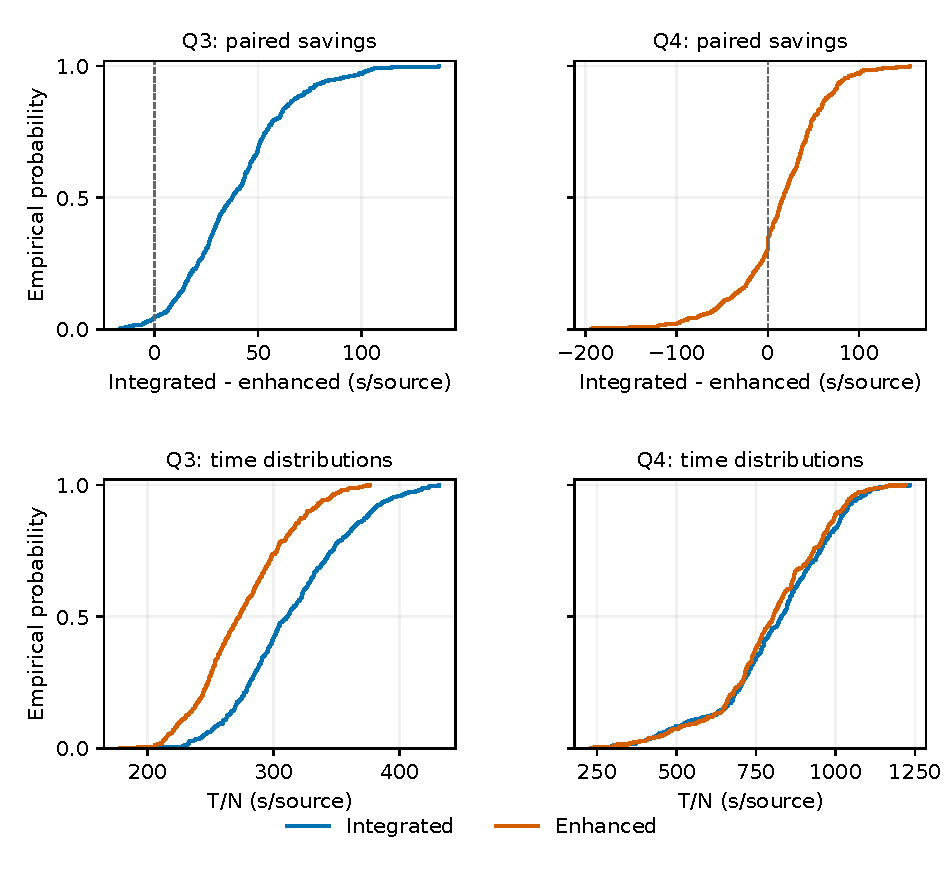
\includegraphics[width=\textwidth]{figures/enhancement_performance.pdf}
\caption{样本外配对差异。正节省代表增强更快，零左侧案例必须保留而不能筛掉。}
\end{figure}

\subsection{收益来自哪里：按每世界每源分解}
表\ref{tab:enhancement-costs}先把每个世界的各项成本除以该世界源数，再对世界求平均。未舍入数据满足计费恒等式；本表逐项保留两位小数后，分项之和与总计可相差0.01秒/源，另有逐动作微秒舍入误差。不能改用所有世界总时间除以总源数，那会增加大源数世界的权重。
\begin{table}[H]\centering\small
\caption{增强前后分项成本，单位为秒/源}\label{tab:enhancement-costs}
\begin{tabular}{@{}>{\raggedright\arraybackslash}p{0.9cm}@{\hspace{0.14cm}}>{\raggedright\arraybackslash}p{1.5cm}@{\hspace{0.14cm}}>{\raggedleft\arraybackslash}p{2.1cm}@{\hspace{0.14cm}}>{\raggedleft\arraybackslash}p{1.8cm}@{\hspace{0.14cm}}>{\raggedleft\arraybackslash}p{1.7cm}@{\hspace{0.14cm}}>{\raggedleft\arraybackslash}p{1.7cm}@{\hspace{0.14cm}}>{\raggedleft\arraybackslash}p{1.7cm}@{\hspace{0.14cm}}>{\raggedleft\arraybackslash}p{2.1cm}@{}}
\toprule
问题 & 策略 & $L/(5N)$ & $5M/N$ & $S/N$ & $3F/N$ & $5K/N$ & 合计/s \\
\midrule
Q3 & 原集成 & 253.14 & 47.77 & 8.88 & 0.18 & 5.00 & 314.98 \\
Q3 & 增强 & 212.66 & 48.79 & 9.05 & 0.17 & 5.00 & 275.68 \\
Q4 & 原集成 & 640.65 & 139.71 & 24.83 & 1.54 & 5.00 & 811.73 \\
Q4 & 增强 & 627.01 & 139.42 & 24.76 & 1.56 & 5.00 & 797.76 \\
\bottomrule
\end{tabular}

\end{table}
Q3收缩环主要减少纯移动，允许稍多的检测来换取更短的路程；这说明最少测向次数不是本题的正确目标。Q4滚动路线保留同样的31点集合，收益来自定位后实际出发位置对后续路线的反馈。只有完整计费式支持这些解释；不以失败清除次数下降单独证明总效率提升。

\subsection{压力分布下的效果边界}
\begin{table}[H]\centering\small
\caption{新增压力检验：每组30对世界，表中节省为基础减增强}\label{tab:enhancement-stress}
\begin{tabular}{@{}>{\raggedright\arraybackslash}p{0.8cm}@{\hspace{0.14cm}}>{\raggedright\arraybackslash}p{1.7cm}@{\hspace{0.14cm}}>{\raggedright\arraybackslash}p{1.7cm}@{\hspace{0.14cm}}>{\raggedleft\arraybackslash}p{2.1cm}@{\hspace{0.14cm}}>{\raggedleft\arraybackslash}p{2.1cm}@{\hspace{0.14cm}}>{\raggedleft\arraybackslash}p{2.1cm}@{\hspace{0.14cm}}>{\raggedleft\arraybackslash}p{1.6cm}@{\hspace{0.14cm}}>{\raggedleft\arraybackslash}p{2.0cm}@{}}
\toprule
问题 & 场景 & 误差 & 原集成/s & 增强/s & 节省/s & 更快/对 & 双全清/对 \\
\midrule
Q3 & 最小半径 & 平滑 & 315.47 & 283.89 & 31.58 & 29/30 & 30/30 \\
Q3 & 最小半径 & 极端 & 321.55 & 290.82 & 30.74 & 28/30 & 30/30 \\
Q3 & 最小半径 & 位置独立 & 316.46 & 284.65 & 31.81 & 30/30 & 30/30 \\
Q3 & 边界朝外 & 平滑 & 304.93 & 329.07 & -24.14 & 5/30 & 30/30 \\
Q3 & 边界朝外 & 极端 & 311.96 & 330.86 & -18.90 & 6/30 & 30/30 \\
Q3 & 边界朝外 & 位置独立 & 307.60 & 332.36 & -24.76 & 2/30 & 30/30 \\
Q3 & 聚集 & 平滑 & 122.56 & 105.31 & 17.26 & 30/30 & 30/30 \\
Q3 & 聚集 & 极端 & 122.77 & 105.41 & 17.36 & 29/30 & 30/30 \\
Q3 & 聚集 & 位置独立 & 122.61 & 105.66 & 16.95 & 29/30 & 30/30 \\
Q4 & 最小半径 & 平滑 & 831.73 & 824.61 & 7.11 & 21/30 & 30/30 \\
Q4 & 最小半径 & 极端 & 832.06 & 819.95 & 12.11 & 17/30 & 30/30 \\
Q4 & 最小半径 & 位置独立 & 823.53 & 823.04 & 0.48 & 18/30 & 30/30 \\
Q4 & 边界朝外 & 平滑 & 879.59 & 875.87 & 3.73 & 17/30 & 30/30 \\
Q4 & 边界朝外 & 极端 & 868.11 & 866.20 & 1.91 & 18/30 & 30/30 \\
Q4 & 边界朝外 & 位置独立 & 881.06 & 875.84 & 5.21 & 19/30 & 30/30 \\
Q4 & 聚集 & 平滑 & 274.33 & 307.89 & -33.57 & 1/30 & 30/30 \\
Q4 & 聚集 & 极端 & 277.62 & 306.33 & -28.72 & 1/30 & 30/30 \\
Q4 & 聚集 & 位置独立 & 280.36 & 316.77 & -36.40 & 1/30 & 30/30 \\
\bottomrule
\end{tabular}

\end{table}
各组的全清首先检验覆盖和终止不变量；正负时间差则反映效率对几何、固定误差场和方向的依赖。不能把普通随机世界的平均改善直接推广为所有压力分布的改善，也不能因某组增时而取消必要的圆外检测。压力场景用于揭示边界，不用于反复调参直至所有行都变为正数。

\subsection{改进结论和实施选择}
本文把“能证明不漏检”与“在样本中平均更快”视为两个独立闸门。候选只有同时保留原有证书、在所有列示运行中完成证书，并在与对照相同的完整计费式下表现稳定，才进入默认策略；否则保留为可复核的负对照，而不是删除其结果。
\begin{table}[H]\centering\small
\caption{候选机制的准入矩阵}
\begin{tabular}{>{\raggedright\arraybackslash}p{2.7cm}>{\raggedright\arraybackslash}p{4.1cm}>{\raggedright\arraybackslash}p{4.9cm}>{\raggedright\arraybackslash}p{1.3cm}}\toprule
机制 & 不变量或安全条件 & 证据与代价 & 决策\\\midrule
Q3收缩环 & 式\eqref{eq:contracted-cover}给出全圆域覆盖，$\rho_{\rm ring}(1200)<1000$ & 150个开发世界筛选，500个样本外配对世界；额外保留31.10米余量 & 采用\\
Q4滚动路径 & 完整31点集合和逐频道检测义务不变 & 500个样本外世界中滚动重排只改变访问顺序；不减少圆外点 & 采用\\
静态2-opt & 点集不变，故安全但不能预见定位支线终点 & 200个同种子世界的完整$T/N$比较中均值增时 & 不采用\\
区间自适应测点 & 正示向评分有保守上界，失败时仍回到光学兜底 & Q4失败次数下降但新增测向和移动，完整时间未稳定改善 & 不采用\\
定向负观测裁剪 & 需维护$(g,R,n)$联合可行集，不能只删位置圆盘 & 当前实现不做未经证明的高维判空 & 不启用\\\bottomrule
\end{tabular}
\end{table}
该矩阵规定的是策略选择条件，而不是强制先扫完骨架再定位。在线程序仍在未完成骨架和已知源之间选择下一任务，保留所有欠缺的频道义务；任何局部评分都不能绕过完整覆盖或把失败清除改写成成功。“优化损失时间”与“证书失效”必须分别处理。

复现时先运行几何验证和终端回归，再运行基础实验与增强实验，随后由资产脚本从JSON重建表格、图形和轨迹，最后编译论文并检查正文页数。该顺序避免人工复制数字，也使每个图表都能追溯到固定代码、输入哈希和种子范围。由于官方测试尚未执行，本节所有“采用”只表示研究程序中的默认实现，不表示已通过正式竞赛测试。


\section{实现与可信度验证}
\subsection{本地环境与决策程序隔离}
合成环境严格执行：不同频道互不影响；有效半径及半平面共同决定可检测性；同一地点同一频道误差固定；距离不超过5米返回近源；清除与发射方向无关；移动按欧氏距离计时；清除不切换测向机频道。

策略只消费与正式接口同形的动作响应，不读取源真值。环境在退出后才提供总数等统计给评价器。实验脚本逐动作用式\eqref{eq:time}重新累计时间，验证成功清除频道不重复、结果数量一致以及每个接受响应的虚拟时刻一致。模拟器自己报告的总时间不是唯一核验依据。

\subsection{几何交叉验证与回归}
\begin{table}[H]\centering\small
\caption{已实际执行的数值与接口检查，采样检查不替代解析证明}
\begin{tabular}{lrl}
\toprule
Numerical / local check & Cases / points & Observed result \\
\midrule
MEC reference & 504 & 1.00e-09 m \\
Bearing containment & 2000 & 4 readings/case \\
Optical cover samples & 4000 & Contained \\
Discovery samples & 2000 & Both geometries \\
Triple-lens samples & 10000 & Reception checked \\
Local HTTP fixture & 1 & Four checks passed \\
\bottomrule
\end{tabular}

\end{table}
独立审查发现并修正了零误差精确示向度的背向射线、同方差信息矩阵的概率解释、极小格距可能导致不可运行的枚举规模以及终端动作越过虚拟期限的问题。前向射线、覆盖见证、收缩环和终端状态均保留了先失败后通过的回归；程序支持格距限定为$[900,999]$米，不接受数值上几乎没有距离余量或会产生天文级点数的实参。

\subsection{HTTP层的可靠性与现实截止}
客户端每个新动作使用唯一请求编号，只在同一逻辑动作传输失败时复用同一编号及相同请求字节。收到完整HTTP响应后才发送下一动作，同时检查HTTP状态与\texttt{accepted}；拒绝响应里的零虚拟时刻不得覆盖当前状态。

本地HTTP故障夹具让首次检测在服务端已执行后只发出半个响应体。客户端恢复时重发同ID，计时只增加一次；附件示例动作序列最终仍为199秒。另一个夹具每0.3秒发一段响应，故意使空闲socket超时不起作用；客户端按0.5秒绝对动作期限退出，实际约0.51秒，且不推进未确认状态、不发送另一动作。

实现采用一个仅负责接收的守护线程与绝对单调时钟等待。超时后的线程即使晚些收到同一动作响应，也不能修改策略状态或发送新动作；客户端保留结果不明状态，禁止推进。它不是并发控制机器狗，只是防止持续慢速响应吞掉全部现实测试窗口。以上两项是本地接口健壮性验证，不代表已与官方模拟器联调。

\section{合成实验、消融和敏感性分析}
\subsection{分布说明及预先隔离的随机种子}
常规世界中，源数在10至16间离散均匀取值，频道无放回抽取，位置按面积均匀分布于圆盘，接收半径在1000至1500米间均匀取值。问题三全为全向源；问题四随机选择至少一个但非全部为定向源，方向均匀分布。这些是合成环境的明示设计，不是对官方测试数据分布的猜测。

误差包含三种固定地点场：有界平滑正弦叠加；随位置哈希取$\pm1^\circ$的极端场；随位置哈希取区间均匀值的场。第三种也不意味着重复同一位置的读数独立。压力场景包括所有半径降至1000米、16个圆周源中15个向外发射，以及16个源聚集在圆边缘附近的35米小圆盘内。

丢信号恢复的开发比较使用种子500000至500099。最终随机配对比较使用600000至600499；恢复消融使用610000至610099；压力场景使用700000起的20个种子；参数扰动使用800000和900000起的30个种子。参数冻结后不根据最终结果反复改动它们。

最终结果文件记录\ExperimentRuns{}次完整运行，包括三种策略在相同世界中的重复运行、压力试验和消融；不能把它称为\ExperimentRuns{}个独立随机世界。主对照的统计单位是每问500个世界中的每个$T/N$，不是把所有世界总时间相加后除以总源数。

\subsection{随机世界的效率比较}
\begin{table}[H]\centering\small
\caption{每问500个同种子世界的三策略比较，时间单位为秒/源；非官方成绩}
\begin{tabular}{lrrrr}
\toprule
Policy & Mean $T/N$ (s) & Median (s) & $p_{90}$ (s) & Complete \\
\midrule
Q3 baseline & 515.57 & 513.83 & 583.17 & 500/500 \\
Q3 batched & 334.31 & 330.38 & 396.93 & 500/500 \\
Q3 integrated & 310.67 & 305.79 & 375.98 & 500/500 \\
Q4 baseline & 1046.74 & 1059.30 & 1282.14 & 500/500 \\
Q4 batched & 810.57 & 824.63 & 1034.11 & 500/500 \\
Q4 integrated & 803.28 & 807.94 & 1032.51 & 500/500 \\
\bottomrule
\end{tabular}

\end{table}

基础集成策略在本组世界的平均单源总耗时为\QThreeTime{}与\QFourTime{}秒，相对逐源往返基线分别降低\QThreeGain\%与\QFourGain\%。这组数据用于基础机制消融；本轮增强的独立样本外结果见第\ref{sec:enhancement}节，两个不同种子组不直接混比均值。

\begin{figure}[H]\centering
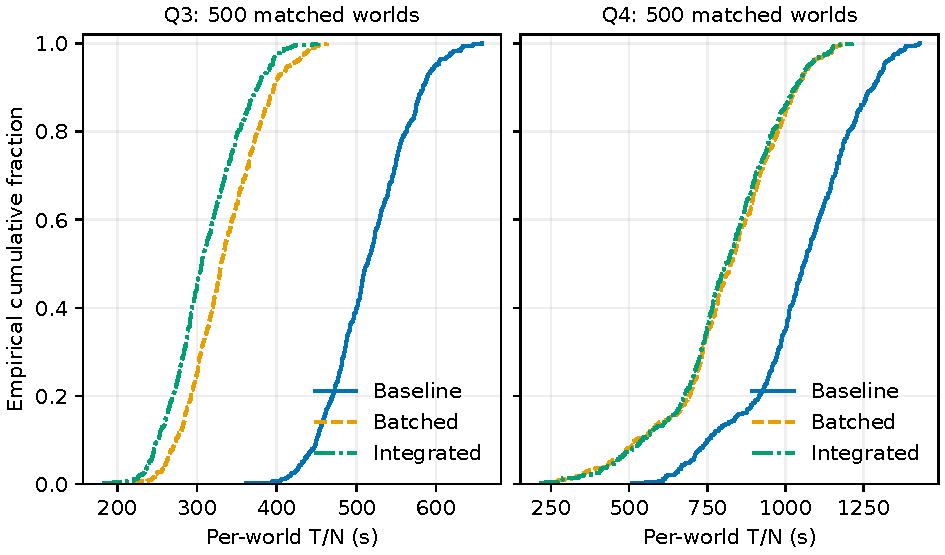
\includegraphics[width=\textwidth]{figures/performance.pdf}
\caption{配对随机世界的单源任务时间分布。不同方案采用相同世界、覆盖与局部定位条件，变化主要来自调度及观测共享。}
\end{figure}

统计程序对基线A与基础集成策略C的逐世界差值$d_j=T_j^{A}/N_j-T_j^{C}/N_j$给出均值和近似95\%区间$\bar d\pm1.96s_d/\sqrt n$。这是蒙特卡洛比较的不确定性，不是未知官方成绩的置信区间。B到C的配对共享消融也单独记录，避免将全部路程收益归因于一个机制。
对任意保持清除证书不变的候选策略，两个同世界运行的时间差必须按完整成本恒等式解释：
\begin{equation}\label{eq:acceptance-threshold}
\Delta T=\frac{\Delta L}{5}+5\Delta M+\Delta S+3\Delta F+5\Delta K.
\end{equation}
定义$\Delta$为候选减对照。真正更快当且仅当$\Delta T<0$；两者均全清时$\Delta K=0$，其他分项的所有有符号变化都应按系数计入。移动增多也可能被检测、切换或失败清除减少抵消。该判据适用于同一世界内比较，不把局部子指标直接等同于完整任务时间。

\begin{figure}[H]\centering
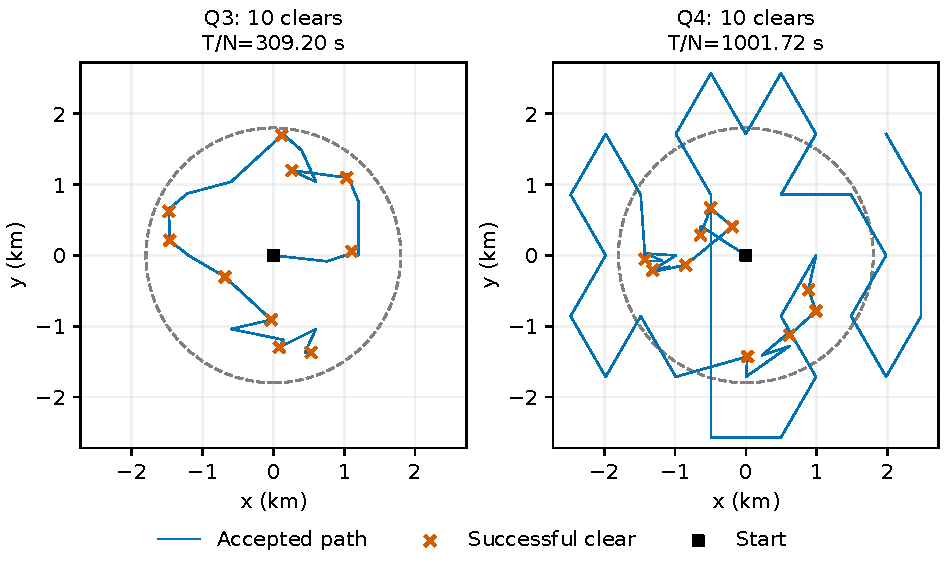
\includegraphics[width=\textwidth]{figures/trajectories.pdf}
\caption{固定示例世界中最终增强策略的完整实际轨迹。点标识的是观察到的成功清除位置，不是程序预先读取的源真值；问题四必须保留圆外搜索。}
\end{figure}

\subsection{极端位置与误差场}
\begin{table}[H]\centering\small
\caption{基础集成策略压力测试：每个问题、场景及误差模式各20次}
\begin{tabular}{llrrr}
\toprule
Geometry & Error field & Q3 mean (s) & Q4 mean (s) & $n$/Q \\
\midrule
Min. radius & Smooth & 336.40 & 877.21 & 20 \\
Min. radius & $\pm1^\circ$ hash & 342.17 & 885.06 & 20 \\
Min. radius & Uniform hash & 335.95 & 882.62 & 20 \\
Outward boundary & Smooth & 308.78 & 870.57 & 20 \\
Outward boundary & $\pm1^\circ$ hash & 303.50 & 880.52 & 20 \\
Outward boundary & Uniform hash & 298.23 & 879.97 & 20 \\
Clustered & Smooth & 107.67 & 352.68 & 20 \\
Clustered & $\pm1^\circ$ hash & 107.74 & 361.78 & 20 \\
Clustered & Uniform hash & 107.89 & 347.05 & 20 \\
\bottomrule
\end{tabular}

\end{table}

所有列示压力运行均完成全清。朝外边界场景尤其检验“圆内无信号不等于无源”和圆外格点是否完整；极端误差场检验是否错误地把多次读数当成可平均消失的噪声；聚集源检验共享停靠与多频道处理。全清结果与解析覆盖结论一致，但不能仅从有限次试验推断所有可能世界都会成功，后者仍依赖前文的集合包含与覆盖证明。

\subsection{丢信号恢复消融}
\begin{table}[H]\centering\small
\caption{问题四同种子恢复消融：每场景100个世界，只有失信号处理开关不同}
\begin{tabular}{lrrrrr}
\toprule
Scenario & $T/N$ off & $T/N$ on & Fails off & Fails on & Pairs \\
\midrule
Random & 807.03 & 803.90 & 68.49 & 8.11 & 100 \\
Min. radius & 839.95 & 813.87 & 96.19 & 8.34 & 100 \\
Outward boundary & 1147.19 & 879.96 & 676.69 & 34.38 & 100 \\
Clustered & 357.32 & 312.94 & 104.63 & 5.13 & 100 \\
\bottomrule
\end{tabular}

\end{table}
\begin{figure}[H]\centering
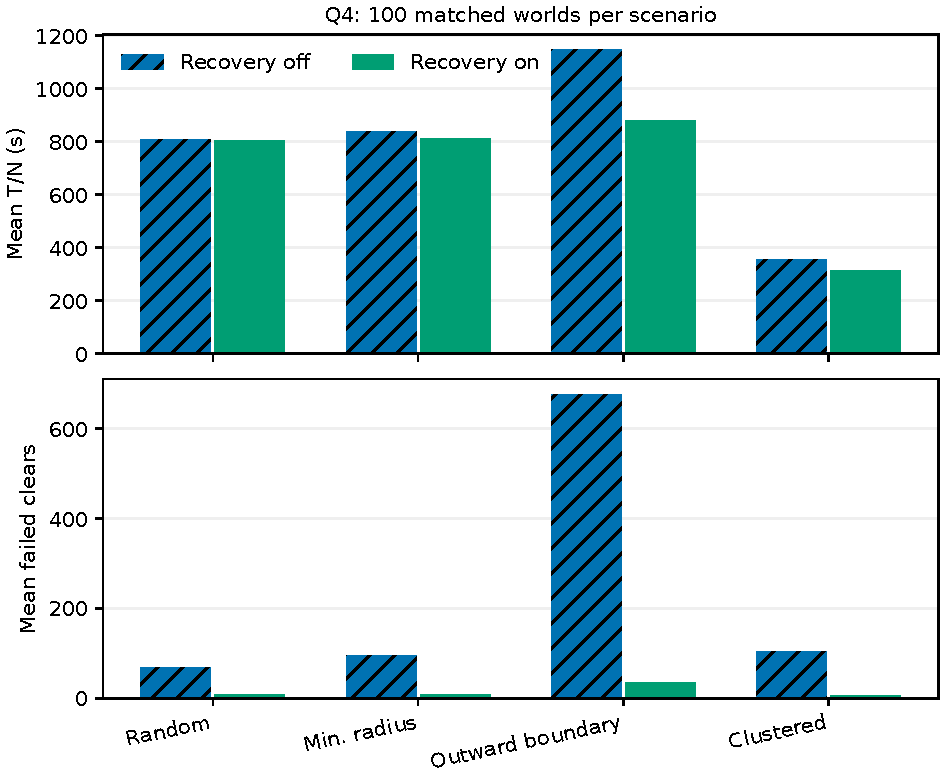
\includegraphics[width=\textwidth]{figures/recovery.pdf}
\caption{有界恢复与直接光学兜底的对照。恢复的主要目的在于降低不利方向场景中大范围光学逐点尝试的开销，而非保证每个普通世界更快。}
\end{figure}

开发阶段发现，单纯尝试中心两侧后立即覆盖整个窄长区域，在朝外边界场景会产生大量失败光学尝试。有限退回和反侧测向针对这一实际问题而增加；恢复失败时仍使用同一全区域后备覆盖，因此增强没有牺牲清除保证。恢复减少失败清除次数不必然按比例降低总时间，因为新的恢复移动与检测同样计费，应以式\eqref{eq:time}的完整结果决定取舍。

\subsection{参数敏感性与局限}
\begin{table}[H]\centering\small
\caption{横向测向尺度和三角格距的独立敏感性试验，各组30次}
\begin{tabular}{llrrr}
\toprule
Problem & Setting & Mean (s) & $p_{90}$ (s) & $n$ \\
\midrule
Q3 & $\lambda=0.12$ & 328.57 & 382.88 & 30 \\
Q3 & $\lambda=0.22$ & 329.04 & 385.26 & 30 \\
Q3 & $\lambda=0.4$ & 329.89 & 385.18 & 30 \\
Q4 & $\lambda=0.12$ & 883.89 & 1067.16 & 30 \\
Q4 & $\lambda=0.22$ & 887.07 & 1060.41 & 30 \\
Q4 & $\lambda=0.4$ & 888.82 & 1066.63 & 30 \\
Q4 & $s=900\,\mathrm{m}$ & 809.26 & 1140.59 & 30 \\
Q4 & $s=950\,\mathrm{m}$ & 736.95 & 1006.62 & 30 \\
Q4 & $s=990\,\mathrm{m}$ & 765.66 & 1005.72 & 30 \\
\bottomrule
\end{tabular}

\end{table}

横向测向尺度围绕默认0.22扰动为0.12、0.40，格距比较900、950、990米。格距越小并不自动越快：它减少到可接收点的最坏距离，却增加骨架节点、检测和移动。离散点集的格层变化和贪心路径会使耗时随参数不完全单调。默认990的选择基于简洁的31点结构与距离余量，不把一次敏感性样本中的最小均值重新命名为普适最优格距。

当前主要局限包括：没有对官方世界分布或误差场进行标定；对负观测的联合位置--方向信息利用不充分；任务评分为滚动启发式而非全局最短路求解；光学覆盖可能包含多边形之外的冗余单元；本地运行的毫秒量级不含官方HTTP往返和界面日志开销。上述局限限制效率结论的外推范围，但不应通过未经证明的概率停止、错误负观测裁剪或隐藏测试真值来消除。

\section{论文结论、交付和后续正式测试}
\subsection{四问的直接结论}
\begin{enumerate}
\item 有界交会多边形的直径由最远顶点对给出；空集、无界集必须另行识别。直径为区域直径的圆不一定能覆盖定位区域，实际一次保证清除应检验最小包围圆半径。
\item 第二点应兼顾距离和交会角。三圆交给出了无需目标距离的全向安全接收候选区域；其内部横向点配合后验可行域评分形成可执行选点算法，但单次读数不足以唯一确定时间最优点。
\item 全向源使用七点覆盖骨架、逐频道完成证书、保守测向定位与有限光学兜底。批量扫描和复用停靠点可以减少重复路程。
\item 混合源使用含18个圆外点的31点三角格，以凸包半平面证书保障任意发射方向的发现；无信号不直接排除附近源，清除则利用方向无关的光学条件。
\end{enumerate}

\subsection{怎样将研究稿升级为可提交成果}
按照官方格式规范，电子版从摘要页开始且不含身份页；摘要原则上不超过一页，摘要之后正文不超过30页，附录另计，附录应包含全部完整可运行代码\cite{format}。本稿不设置目录，附录代码与支撑材料相对应，配套复现说明列出环境和命令。

官方模拟器已经明确搁置，因此本稿\textbf{不填写虚构的三次正式测试表}。恢复可用后，应先完成对应问题的不限次官方演练，核对成功比例、全部动作计时和现实耗时；固定程序后分别进行问题三、四的三次正式测试。从界面抄录实际案例编码、实际清除数、平均总耗时和程序时间，从模拟器导出六份原名加密日志，并核对上传状态。这些日志不能由本地JSONL替代。

官方协议请求日志含参赛队号，只是私有工作材料，不能未经脱敏放入匿名论文支撑包。官方规定要求AI输出逐项人工审查、参赛队主导核心建模\cite{airule}；多代理审查或自动测试都不是人工核验。完成上述环节之前，交付状态必须保持研究复核版，而非“保证获奖”或“已经满足提交要求”。

\section*{AI工具使用声明}
本研究过程中使用了AI工具，参与核心模型推导、代码实现、实验设计、结果整理、独立自动审查及论文写作，详细过程见支撑材料中的《AI工具使用详情》。本稿尚无真实参赛队完成逐项人工核验的记录，不将自动审查写作人工审查；该声明用于如实披露研究过程，不能替代正式提交前应完成的参赛队责任。

\begin{thebibliography}{9}
\raggedright
\bibitem{problem} 全国大学生数学建模竞赛组委会. 2026年高教社杯全国大学生数学建模竞赛B题：无线电干扰源的快速自动定位与清除，以及附件1、附件2[Z]. 2026. \url{https://www.mcm.edu.cn/html_cn/node/27b6e148f8113f09b0269f64a02629fb.html}.
\bibitem{welzl} Welzl E. Smallest enclosing disks (balls and ellipsoids)[C]//New Results and New Trends in Computer Science. Lecture Notes in Computer Science, 555. Springer, 1991: 359--370. DOI: 10.1007/BFb0038202.
\bibitem{format} 全国大学生数学建模竞赛组委会. 全国大学生数学建模竞赛论文格式规范（2026年修订稿）[EB/OL]. \url{https://www.mcm.edu.cn/html_cn/node/4cd596519c9eb9fbd866398f6df0caa3.html}.
\bibitem{airule} 全国大学生数学建模竞赛组委会. 全国大学生数学建模竞赛人工智能工具使用规定（2026年试行）[EB/OL]. \url{https://www.mcm.edu.cn/html_cn/node/fef94648f2836ab6cc81586f4c38512b.html}.
\end{thebibliography}
\label{endbody}
\clearpage
\appendix
% 本文件为 paper.tex 使用的附录片段；主文件负责加载 listings 宏包。
\section{匿名复现附录}
本附录只列出匿名包中实际存在、可供复现使用的源文件。代码路径均相对于本文件所在的\texttt{report/}目录；结果路径均相对于匿名包项目根目录；不含个人绝对路径、队伍身份或私有凭据。主文件应在导言区加载\texttt{listings}并设置合适的Python样式。

\subsection{运行与验证源代码}
\lstinputlisting[language=Python,caption={规划器与恢复策略}]{../planner.py}
\lstinputlisting[language=Python,caption={实验主程序}]{../experiments.py}
\lstinputlisting[language=Python,caption={统一运行入口}]{../run.py}
\lstinputlisting[language=Python,caption={几何计算}]{../geometry.py}
\lstinputlisting[language=Python,caption={几何验证}]{../verify_geometry.py}
\lstinputlisting[language=Python,caption={问题一原始交会区域分类与直径}]{../intersection.py}
\lstinputlisting[language=Python,caption={覆盖与采样工具}]{../coverage.py}
\lstinputlisting[language=Python,caption={环境与模拟器接口}]{../environment.py}
\lstinputlisting[language=Python,caption={第二交点计算}]{../second_point.py}
\lstinputlisting[language=Python,caption={恢复策略比较}]{../compare_recovery.py}
\lstinputlisting[language=Python,caption={HTTP 客户端}]{../client.py}
\lstinputlisting[language=Python,caption={HTTP 验证}]{../verify_http.py}
\lstinputlisting[language=Python,caption={官方运行入口（仅获授权后使用）}]{../official_run.py}
\lstinputlisting[language=Python,caption={数据驱动图表与轨迹生成}]{../make_assets.py}
\lstinputlisting[language=Python,caption={PDF逐页渲染与结构审计}]{../audit_pdf.py}
\lstinputlisting[language=Python,caption={匿名材料打包与解压复现验证}]{../package.py}
\lstinputlisting[language=Python,caption={区间评分自适应测点候选}]{../active_policy_candidate.py}
\lstinputlisting[language=Python,caption={骨架路由候选}]{../route_policy_candidate.py}
\lstinputlisting[language=Python,caption={路由候选对照实验}]{../compare_routes.py}
\lstinputlisting[language=Python,caption={自适应测点对照实验}]{../compare_probes.py}
\lstinputlisting[language=Python,caption={超时终端状态回归}]{../verify_terminal.py}
\lstinputlisting[language=Python,caption={环半径与滚动调度开发比较}]{../develop_anchors.py}
\lstinputlisting[language=Python,caption={增强策略样本外实验}]{../enhancements.py}
\lstinputlisting[language=Python,caption={Q3环半径筛选与新世界确认}]{../ring_sweep.py}
\lstinputlisting[language=Python,caption={增强几何及区间评分交叉验证}]{../verify_refinements.py}
\lstinputlisting[language=Python,caption={31格点不可删反例验证}]{../verify_coverage_limits.py}
\lstinputlisting[language=Python,caption={增强策略图表生成}]{../make_enhancement_assets.py}
\lstinputlisting[language=TeX,caption={覆盖上界理论片段}]{../coverage_limits.tex}
\lstinputlisting[language=TeX,caption={默认有限时间证明片段}]{bound_proof.tex}
\lstinputlisting[language=TeX,caption={样本外增强分析片段}]{enhancements.tex}

\subsection{匿名文件清单与结果接口}
\begin{longtable}{p{0.60\textwidth}p{0.32\textwidth}}
\toprule 文件或目录 & 用途\\\midrule
\path{results/final_experiments.json} & 4430次最终合成运行\\
\path{results/enhancement_experiments.json} & 3080次样本外增强运行\\
\path{results/ring_sweep.json} & Q3环半径开发筛选及样本外配对证据\\
\path{results/coverage_limits.json} & 全部31点不可删构造\\
\path{results/refinement_verification.json} & 收缩环与角区间上界验证\\
\path{results/geometry_verification.json} & 几何交叉核验与回归\\
\path{results/intersection_verification.json} & 原始交会区域三种状态\\
\path{results/http_verification.json} & 幂等重试与计时验证\\
\path{results/http_deadline_verification.json} & 慢速响应绝对期限验证\\
\path{results/second_point_example.json} & 第二测点候选评分\\
\path{results/recovery_development.json} & 恢复策略开发对照\\
\path{results/visual_review.json} & PDF逐页视觉检查记录\\
\path{results/enhancement_review.json} & 增强策略独立审阅记录\\
\path{results/paper_review.json} & 非官方自动审阅记录\\
\path{results/final_review.json} & 新结论与新世界证据的最终独立审查\\
\path{report/generated/} & 自动数字、表格与轨迹证据\\
\path{report/figures/} & 基础及增强矢量图\\
\path{report/ai_usage.tex} & AI使用详情源文件\\
\path{reproduce.txt}、\path{requirements.txt} & 命令、环境及依赖\\
\path{MANIFEST.json} & 支撑包内文件校验值\\
\path{results/route_candidate_comparison.json} & 路由候选负结果\\
\path{results/adaptive_candidate_comparison.json} & 自适应测点候选负结果与子指标\\
\path{results/terminal_verification.json} & 虚拟/现实期限终端回归\\
\path{theory_additions.txt}、\path{paper_expansion.txt} & 独立理论草稿\\
\path{report/generated/coverage_limits_table.tex} & 不可删性汇总表\\
\bottomrule
\end{longtable}
图表由\path{make_assets.py}和\path{make_enhancement_assets.py}读取对应JSON生成，完整代码如上。\path{audit_pdf.py}渲染全部页面并检查文字边界；\path{package.py --verify}解压支撑包，重新运行计算和编译，不以原目录存在文件代替解压可复现性。

含有官方 \texttt{robot\_id} 的私有 HTTP 日志不进入匿名包；如正式流程要求提交官方加密导出，应保持官方给出的原文件名和原始字节，不在公开包中复制或改写。官方模拟器尚未运行，故本附录不提供官方输出。

\end{document}
